% ============================================================
%  chapter11_slides.tex  --  Chapter 11: Duality
%  Algorithms for Optimization, 2nd ed. (2026)
%  Kochenderfer & Wheeler  --  MIT Press
%
%  Compile:  pdflatex -interaction=nonstopmode chapter11_slides.tex  (twice)
% ============================================================
\documentclass[aspectratio=169,10pt]{beamer}

\usetheme{Madrid}
\usecolortheme{seahorse}

\usepackage{amsmath,amssymb,amsfonts}
\usepackage{bm}
\usepackage{graphicx}
\usepackage{booktabs}
\usepackage{listings}
\usepackage{xcolor}
\usepackage{tikz}
\usetikzlibrary{arrows.meta,positioning,shapes.geometric}
\usepackage{microtype}
\usepackage{multicol}
\usepackage{array}

\graphicspath{{figures/}}

% ---- listings Python style ----
\lstdefinestyle{python}{
  language=Python,
  basicstyle=\ttfamily\scriptsize,
  numbers=left,
  numberstyle=\tiny\color{gray},
  stepnumber=1,
  numbersep=5pt,
  frame=single,
  backgroundcolor=\color{gray!7},
  keywordstyle=\color{blue!70!black}\bfseries,
  commentstyle=\color{green!50!black}\itshape,
  stringstyle=\color{orange!80!black},
  breaklines=true,
  showstringspaces=false,
  tabsize=4,
}

\setbeamertemplate{footline}[frame number]
\setbeamertemplate{navigation symbols}{}

% shorthand
\newcommand{\bx}{\mathbf{x}}
\newcommand{\by}{\mathbf{y}}
\newcommand{\bz}{\mathbf{z}}
\newcommand{\bu}{\mathbf{u}}
\newcommand{\bv}{\mathbf{v}}
\newcommand{\bw}{\mathbf{w}}
\newcommand{\bg}{\mathbf{g}}
\newcommand{\bh}{\mathbf{h}}
\newcommand{\bA}{\mathbf{A}}
\newcommand{\bB}{\mathbf{B}}
\newcommand{\bI}{\mathbf{I}}
\newcommand{\bb}{\mathbf{b}}
\newcommand{\bc}{\mathbf{c}}
\newcommand{\bmu}{\boldsymbol{\mu}}
\newcommand{\blam}{\boldsymbol{\lambda}}
\newcommand{\R}{\mathbb{R}}
\newcommand{\calL}{\mathcal{L}}
\newcommand{\calD}{\mathcal{D}}
\newcommand{\grad}{\nabla}
\newcommand{\bp}{\mathbf{p}}

% ============================================================
\title[Chapter 11: Duality]{Chapter 11: Duality}
\subtitle{Algorithms for Optimization, 2nd ed.\ (2026)}
\author{Kochenderfer \& Wheeler}
\institute{MIT Press}
\date{}

% ============================================================
\begin{document}

\begin{frame}
  \titlepage
\end{frame}

\begin{frame}{Outline}
  \tableofcontents
\end{frame}

% ============================================================
\section{11.1 Dual Problem}
% ============================================================

\begin{frame}[allowframebreaks]{Motivation: Why Duality?}

Most optimisation problems start as a \emph{primal} problem: minimise some
objective subject to constraints.  Duality is a powerful theoretical tool that
lets us construct a companion \emph{dual} problem whose solution always
provides a guaranteed lower bound on the primal optimal value.

\begin{columns}
  \begin{column}{0.55\textwidth}
    The key benefits of working with duality are:

    \medskip
    \textbf{(1) Verification:} when the dual optimal value equals the primal
    optimal value --- a situation called \emph{strong duality} --- solving
    either problem gives us the answer to both, and we can certify optimality
    without exhaustive search.

    \medskip
    \textbf{(2) Algorithm design:} many of the most efficient practical
    solvers --- interior-point methods, ADMM (Alternating Direction Method of
    Multipliers), and distributed optimisation algorithms --- are built
    directly on the dual structure of the problem.

    \medskip
    \textbf{(3) Sensitivity analysis:} the dual variables (also called
    Lagrange multipliers, explained below) tell us how much the optimal
    objective value would change if we tightened or relaxed each constraint
    by a small amount.
  \end{column}
  \begin{column}{0.42\textwidth}
    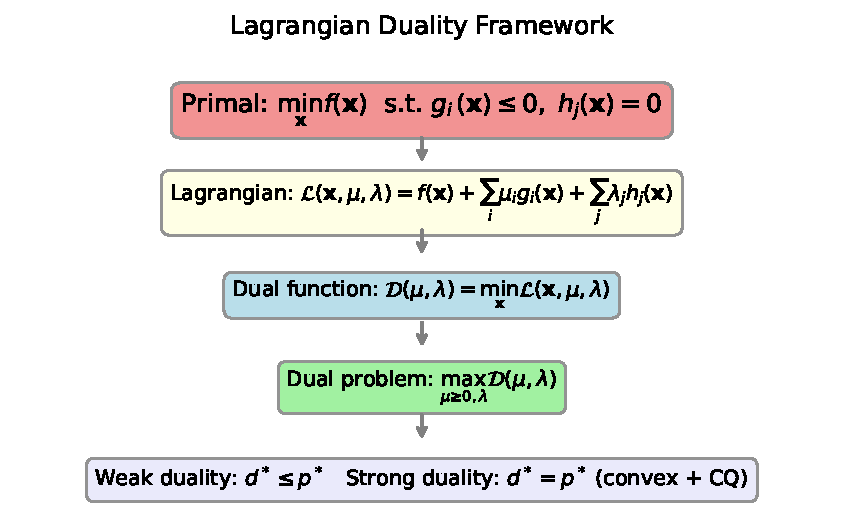
\includegraphics[width=\linewidth]{fig_lagrangian_overview.pdf}
  \end{column}
\end{columns}

\begin{alertblock}{Key Insight}
  The dual problem is always a \emph{concave maximisation} problem, regardless
  of whether the primal is convex.  This means dual ascent algorithms always
  converge --- a very useful property.
\end{alertblock}

\end{frame}

% ----
\begin{frame}[allowframebreaks]{The Generalised Lagrangian}

  We begin with the most general form of a constrained optimisation problem.
  Suppose we want to minimise an objective $f(\bx)$ subject to inequality
  constraints $\bg(\bx) \le \mathbf{0}$ and equality constraints
  $\bh(\bx) = \mathbf{0}$:

  \begin{block}{General Constrained Problem}
    \[
      \min_{\bx}\; f(\bx) \quad \text{subject to} \quad
      \bg(\bx) \le \mathbf{0},\quad \bh(\bx) = \mathbf{0}
    \]
    where $\bx \in \R^n$ (x, an $n$-dimensional real vector) is the vector of
    decision variables we are optimising over.
  \end{block}

  \medskip
  The central idea of duality is to ``relax'' the constraints by moving them
  into the objective function, weighted by penalty multipliers.  The result
  is the \textbf{Generalised Lagrangian} (named after the mathematician
  Joseph-Louis Lagrange):

  \begin{block}{Generalised Lagrangian}
    \[
      \calL(\bx, \bmu, \blam)
      \;=\; f(\bx)
      \;+\; \sum_i \mu_i\, g_i(\bx)
      \;+\; \sum_j \lambda_j\, h_j(\bx)
    \]
  \end{block}

  \begin{block}{Notation}
    \begin{itemize}
      \item $\bx \in \R^n$: the \emph{primal} (design) variables --- the
            quantities we are trying to find.
      \item $\bmu \ge \mathbf{0}$ (mu, pronounced ``myoo'', a bold Greek
            letter): a vector of \emph{inequality multipliers}, one per
            inequality constraint $g_i(\bx) \le 0$.  Each $\mu_i \ge 0$
            must be non-negative.
      \item $\blam \in \R^p$ (lambda, pronounced ``lam-da'', a bold Greek
            letter): a vector of \emph{equality multipliers}, one per
            equality constraint $h_j(\bx) = 0$.  These can be any sign.
      \item $g_i(\bx)$: the $i$-th inequality constraint function evaluated
            at $\bx$; the constraint requires this to be $\le 0$.
      \item $h_j(\bx)$: the $j$-th equality constraint function; the
            constraint requires this to equal $0$ exactly.
      \item $\sum_i$ (Sigma, meaning ``sum over index $i$''): we add up one
            term for each inequality constraint.
    \end{itemize}
  \end{block}

  \begin{alertblock}{How to Read This Formula}
    Think of the Lagrangian as an ``augmented objective.''  When $\bx$
    satisfies all inequality constraints, $g_i(\bx) \le 0$, and since
    $\mu_i \ge 0$, the penalty terms $\mu_i g_i(\bx)$ are non-positive ---
    they do not inflate the objective.  But if $\bx$ violates a constraint
    (so $g_i(\bx) > 0$), the penalty $\mu_i g_i(\bx)$ becomes \emph{positive},
    pushing the Lagrangian above $f(\bx)$ and discouraging infeasibility.
    The multipliers $\mu_i$ and $\lambda_j$ are also called \textbf{dual
    variables} because they become the variables of the dual problem.
  \end{alertblock}

\end{frame}

% ----
\begin{frame}[allowframebreaks]{Primal and Dual Problems}

  Starting from the Lagrangian $\calL(\bx, \bmu, \blam)$, we can recover the
  original constrained problem by a clever minimax trick, and then derive the
  dual by swapping the order of min and max.

  \begin{block}{Primal Problem}
    \[
      p^* \;=\; \min_{\bx}\; \max_{\bmu \ge \mathbf{0},\;\blam}\;
      \calL(\bx, \bmu, \blam)
    \]
    Here $p^*$ (p-star) is the \emph{optimal primal value} --- the lowest
    possible value of $f(\bx)$ subject to all constraints.
  \end{block}

  Why does this recover the original problem?  If $\bx$ violates any
  inequality constraint, then $g_i(\bx) > 0$ for some $i$, and we can send
  $\mu_i \to +\infty$, making the inner maximum $+\infty$.  An outer
  minimisation over $\bx$ will never choose an infeasible point.  For
  feasible $\bx$, $g_i(\bx) \le 0$, the best multipliers set $\mu_i = 0$
  and $\lambda_j = 0$, so the maximum equals $f(\bx)$.

  \framebreak

  \begin{block}{Dual Function}
    \[
      \calD(\bmu, \blam) \;=\; \min_{\bx}\; \calL(\bx, \bmu, \blam)
    \]
    For fixed multipliers $(\bmu, \blam)$, this is the \emph{minimum value
    of the Lagrangian over all $\bx$} (with no constraints on $\bx$).
  \end{block}

  The dual function $\calD$ (script D) has a remarkable property: it is
  always \textbf{concave} in $(\bmu, \blam)$, even when the original problem
  is non-convex.  This is because it is a pointwise minimum of affine
  (linear) functions of $(\bmu, \blam)$, and a minimum of affines is
  always concave.

  \begin{block}{Dual Problem}
    \[
      d^* \;=\; \max_{\bmu \ge \mathbf{0},\;\blam}\; \calD(\bmu, \blam)
    \]
    Here $d^*$ (d-star) is the \emph{optimal dual value} --- the highest
    value of the dual function achievable over all valid multipliers.
  \end{block}

  \begin{alertblock}{Key Insight}
    We have transformed a minimisation problem into a maximisation problem.
    The dual problem is always concave, which makes it easier to solve with
    gradient ascent methods --- they are guaranteed to find the global maximum
    of a concave function.
  \end{alertblock}

\end{frame}

% ----
\begin{frame}[allowframebreaks]{Weak and Strong Duality}

  \begin{columns}
    \begin{column}{0.55\textwidth}
      \begin{block}{Weak Duality (always true)}
        \[
          d^* \;\le\; p^*
        \]
        The dual optimal value is \emph{always} a lower bound on the
        primal optimal value.  This holds regardless of convexity or
        any other assumption.
      \end{block}

      The difference $p^* - d^* \ge 0$ is called the \textbf{duality gap}.
      A large gap means the dual bound is loose; a gap of zero means we
      have found exact optimality certificates.

      \medskip
      \begin{block}{Strong Duality}
        \[
          d^* \;=\; p^*
        \]
        The gap is zero --- the dual and primal optimal values coincide.
        Strong duality holds for \textbf{convex} problems that satisfy a
        \emph{constraint qualification}, such as:

        \smallskip
        \textbf{Slater's condition:} there exists at least one $\hat{\bx}$
        in the interior of the feasible set, meaning $g_i(\hat{\bx}) < 0$
        strictly for all $i$ (strictly feasible point).
      \end{block}
    \end{column}
    \begin{column}{0.42\textwidth}
      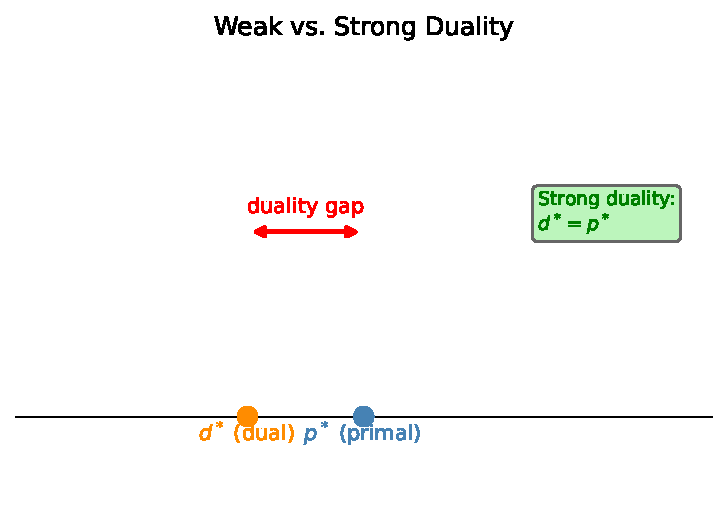
\includegraphics[width=\linewidth]{fig_duality_gap.pdf}
    \end{column}
  \end{columns}

  \begin{alertblock}{How to Read This}
    Think of the primal value $p^*$ as the ``true answer'' and the dual
    value $d^*$ as a ``certificate'' that no solution can do better.  Weak
    duality says the certificate can never exceed the truth.  Strong duality
    says the certificate is tight --- we can verify optimality exactly.
    In practice, algorithms drive the duality gap to near-zero as a
    stopping criterion.
  \end{alertblock}

\end{frame}

% ----
\begin{frame}[allowframebreaks]{Example 11.1: Dual Function as Lower Bound}

  This example makes the abstract notion of ``lower bound'' concrete.

  \begin{columns}
    \begin{column}{0.52\textwidth}
      \textbf{The problem:} minimise $\sin(x)$ subject to $x^2 \le 1$
      (so $x$ must lie in the interval $[-1, 1]$).

      \medskip
      The minimum of $\sin(x)$ on $[-1, 1]$ occurs at $x^* = -1$,
      giving $p^* = \sin(-1) \approx -0.841$.

      \medskip
      \textbf{Constructing the Lagrangian:} the single inequality constraint
      is $g(x) = x^2 - 1 \le 0$, so the Lagrangian is:
      \[
        \calL(x, \mu) \;=\; \sin(x) \;+\; \mu\,(x^2 - 1)
      \]
      where $\mu \ge 0$ (mu) is the scalar inequality multiplier.

      \medskip
      \textbf{Primal (minimax):}
      \[
        p^* \;=\; \min_x \max_{\mu \ge 0} \bigl[\sin(x) + \mu(x^2 - 1)\bigr]
      \]

      \textbf{Dual (maximin):}
      \[
        d^* \;=\; \max_{\mu \ge 0} \min_x \bigl[\sin(x) + \mu(x^2 - 1)\bigr]
      \]

      Each curve in the figure shows $\calL(x, \mu)$ for a fixed value of
      $\mu$.  The minimum of each curve (shown in purple) lies \emph{below}
      $p^* \approx -0.841$, illustrating weak duality.  Strong duality
      holds here: the dual optimal value also equals $-0.841$.
    \end{column}
    \begin{column}{0.46\textwidth}
      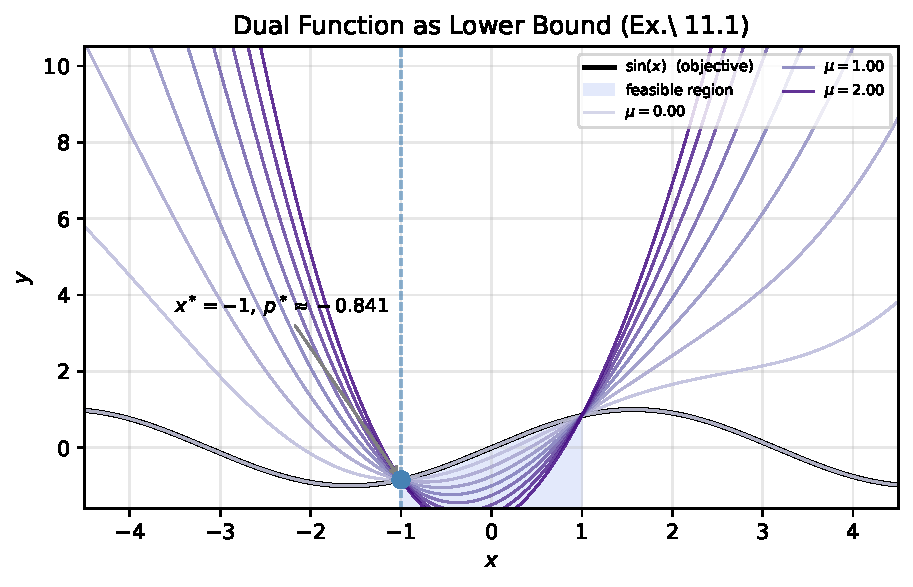
\includegraphics[width=\linewidth]{fig_dual_lower_bound.pdf}
    \end{column}
  \end{columns}

\end{frame}

% ----
\begin{frame}[allowframebreaks]{Example 11.2: Lagrangian Duality with Equality Constraint}

  Here we work through a two-variable problem with an equality constraint,
  deriving the dual function explicitly and verifying strong duality.

  \textbf{The problem:}
  \[
    \min_{\bx}\; x_1 + x_2 + x_1 x_2
    \quad \text{subject to} \quad x_1^2 + x_2^2 = 1
  \]
  The constraint forces $(x_1, x_2)$ to lie on the unit circle (the set of
  points at distance 1 from the origin).

  \medskip
  \textbf{Constructing the Lagrangian:} the single equality constraint is
  $h(x_1, x_2) = x_1^2 + x_2^2 - 1 = 0$, so:
  \[
    \calL(x_1, x_2, \lambda)
    \;=\; x_1 + x_2 + x_1 x_2
    \;+\; \lambda\,(x_1^2 + x_2^2 - 1)
  \]
  where $\lambda$ (lambda, pronounced ``lam-da'') is the equality multiplier
  (unrestricted in sign).

  \medskip
  \textbf{Finding critical points} by setting partial derivatives to zero:
  \[
    \frac{\partial \calL}{\partial x_1} = 1 + x_2 + 2\lambda x_1 = 0,
    \qquad
    \frac{\partial \partial \calL}{\partial x_2} = 1 + x_1 + 2\lambda x_2 = 0,
    \qquad
    x_1^2 + x_2^2 = 1
  \]
  Here $\frac{\partial \calL}{\partial x_1}$ means the partial derivative
  of $\calL$ with respect to $x_1$, i.e.\ the rate of change of $\calL$
  as $x_1$ varies while $x_2$ and $\lambda$ are held fixed.

  \framebreak

  Solving the three equations simultaneously yields \textbf{four critical
  points}:

  \begin{center}
  \begin{tabular}{cccl}
    \toprule
    $x_1$ & $x_2$ & $\lambda$ & Objective $f(\bx)$ \\
    \midrule
    $-1$ & $0$ & $1/2$ & $-1$ \quad (global minimum) \\
    $0$ & $-1$ & $1/2$ & $-1$ \quad (global minimum) \\
    $\dfrac{\sqrt{2}+1}{\sqrt{2}+2}$ & $\dfrac{\sqrt{2}+1}{\sqrt{2}+2}$ &
      $\frac{1}{2}(-1-\sqrt{2})$ & $\approx 1.914$ \quad (global maximum) \\
    $\dfrac{\sqrt{2}-1}{\sqrt{2}-2}$ & $\dfrac{\sqrt{2}-1}{\sqrt{2}-2}$ &
      $\frac{1}{2}(-1+\sqrt{2})$ & $\approx -0.914$ \quad (saddle point) \\
    \bottomrule
  \end{tabular}
  \end{center}

  The optimal primal value is $p^* = -1$, achieved at $(-1, 0)$ and $(0, -1)$.

  \framebreak

  \textbf{Deriving the dual function:} substituting $u = x_1 + x_2$
  and $v = x_1 - x_2$ transforms the Lagrangian into:
  \[
    \calL \;=\; \tfrac{1}{4}(2\lambda + 1)\,u^2 \;+\; u
               \;+\; \tfrac{1}{4}(2\lambda - 1)\,v^2 \;-\; \lambda
  \]
  Minimising over $u$ and $v$ gives the dual function:

  \begin{block}{Dual Function $\calD(\lambda)$}
    \[
      \calD(\lambda) \;=\;
      \begin{cases}
        -\!\left(\dfrac{1}{2\lambda + 1} + \lambda\right) & \lambda \ge \tfrac{1}{2} \\[6pt]
        -\infty & \text{otherwise}
      \end{cases}
    \]
  \end{block}

  \begin{columns}
    \begin{column}{0.50\textwidth}
      The dual function equals $-\infty$ for $\lambda < 1/2$ because the
      quadratic in $v$ becomes unbounded below.  For $\lambda \ge 1/2$,
      we can minimise the Lagrangian, and the maximum of $\calD(\lambda)$
      occurs at $\lambda^* = 1/2$, giving $d^* = -(1/2 + 1/2) = -1 = p^*$.

      \medskip
      This confirms \textbf{strong duality}: $d^* = p^* = -1$.
    \end{column}
    \begin{column}{0.48\textwidth}
      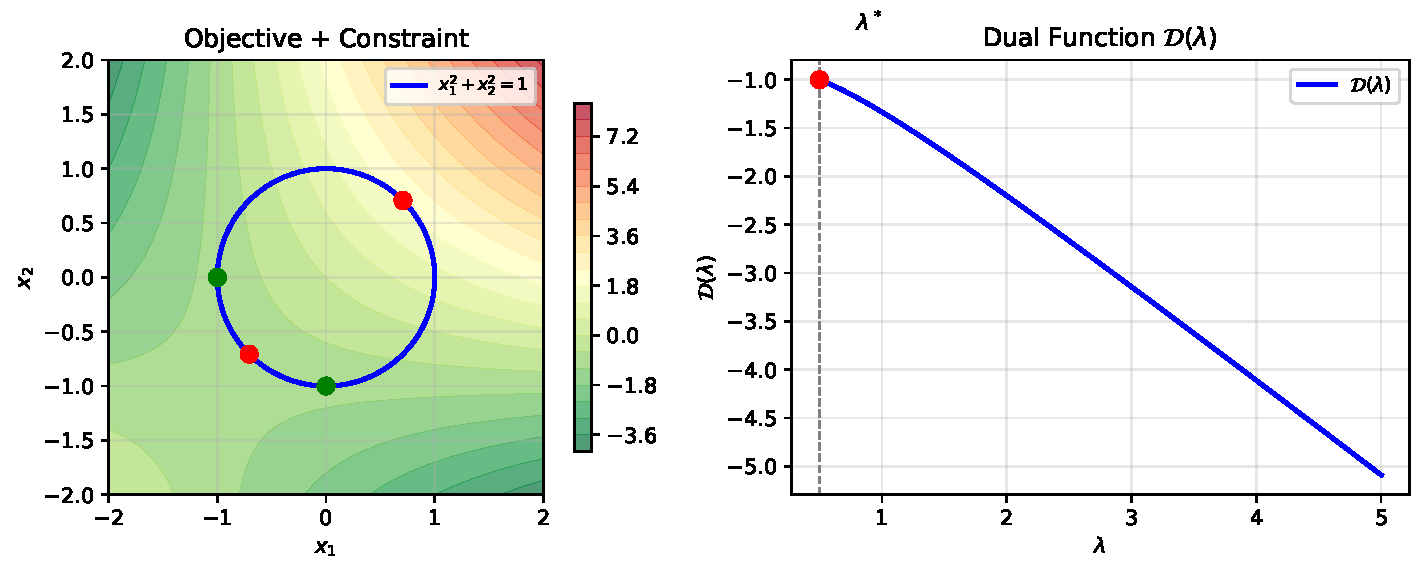
\includegraphics[width=\linewidth]{fig_dual_function_ex2.pdf}
    \end{column}
  \end{columns}

\end{frame}

% ============================================================
\section{11.2 Primal-Dual Methods}
% ============================================================

\begin{frame}[allowframebreaks]{Primal-Dual Interior-Point: Motivation}

  Primal-dual interior-point methods are among the most powerful algorithms
  for solving convex constrained optimisation problems.  The idea is to
  update the primal variables $\bx$ and the dual variables $\bmu$ (mu)
  \emph{simultaneously} at each iteration, rather than alternating between
  them.  This joint update leads to very fast convergence in practice.

  \medskip
  We focus on the inequality-constrained problem:
  \begin{block}{Inequality-Constrained Problem}
    \[
      \min_{\bx}\; f(\bx)
      \quad \text{subject to} \quad
      \bg(\bx) \le \mathbf{0}
    \]
    where $\bg(\bx) = [g_1(\bx), \ldots, g_m(\bx)]^\top$ is the vector of
    $m$ inequality constraint functions.
  \end{block}

  \textbf{Step 1 --- Replace constraints with a log-barrier:}  instead of
  enforcing $g_i(\bx) \le 0$ directly, we add a \emph{logarithmic barrier}
  that blows up as $\bx$ approaches the constraint boundary:
  \begin{block}{Log-Barrier Problem}
    \[
      \min_{\bx}\; f(\bx) - \frac{1}{\rho} \sum_{i=1}^{m} \log(-g_i(\bx))
    \]
  \end{block}

  \begin{block}{Notation}
    \begin{itemize}
      \item $\rho$ (rho, pronounced ``roe''): a positive penalty parameter
            that controls how strongly the barrier enforces constraints.
            As $\rho \to \infty$, the barrier becomes more and more
            concentrated at the boundary.
      \item $\log(\cdot)$: the natural logarithm.  When $g_i(\bx)$ is
            negative (feasible), $-g_i(\bx)$ is positive, so
            $\log(-g_i(\bx))$ is finite.  As $g_i(\bx) \to 0$ from below,
            $-g_i(\bx) \to 0^+$ and $\log(-g_i(\bx)) \to -\infty$,
            creating a barrier wall at the boundary.
      \item $\frac{1}{\rho}$: the barrier weight.  A small weight (large
            $\rho$) means the barrier is almost invisible far from the
            boundary, so the solution stays close to the true constrained
            optimum.
    \end{itemize}
  \end{block}

  \framebreak

  \textbf{Step 2 --- Interpret the optimality condition:}
  setting the gradient of the barrier objective to zero gives:
  \[
    \mathbf{0} \;=\; \grad f(\bx^*) \;+\;
    \sum_{i=1}^m \underbrace{\frac{-1}{\rho\, g_i(\bx^*)}}_{\mu_i^*}\,
    \grad g_i(\bx^*)
  \]
  Here $\grad$ (nabla, the del or gradient operator) denotes the vector of
  partial derivatives.  We can define $\mu_i^* = -1/(\rho\, g_i(\bx^*))$,
  which is automatically positive since $g_i(\bx^*) < 0$ for a strictly
  interior point.  This recovers the KKT stationarity condition:
  \[
    \mathbf{0} \;=\; \grad f(\bx^*) + \sum_{i=1}^m \mu_i^*\, \grad g_i(\bx^*)
  \]

  \textbf{Step 3 --- Duality gap:}
  one can show that the duality gap at the barrier solution equals
  $m/\rho$, where $m$ is the number of constraints.  As $\rho \to \infty$,
  the gap shrinks to zero, confirming convergence to the true constrained
  optimum.

  \begin{alertblock}{Key Insight}
    By increasing $\rho$ gradually, the log-barrier solution tracks the true
    constrained optimum ever more closely.  Primal-dual methods do not solve
    a sequence of separate barrier problems; instead, they use a Newton step
    that simultaneously drives both the primal residual and the duality gap
    to zero.
  \end{alertblock}

\end{frame}

% ----
\begin{frame}[allowframebreaks]{Primal-Dual System and Newton Step}

  The primal-dual method seeks to satisfy both \emph{stationarity} and
  \emph{complementary slackness} simultaneously.  It does this by defining
  a residual vector $\mathbf{r}$ that packages all the optimality conditions,
  and then applying a Newton step to drive $\mathbf{r}$ to zero.

  \begin{block}{Residual Vector $\mathbf{r}(\bx, \bmu, \rho)$}
    \[
      \mathbf{r}(\bx, \bmu, \rho) \;=\;
      \begin{bmatrix}
        \grad f(\bx) + \displaystyle\sum_i \mu_i\, \grad g_i(\bx) \\[6pt]
        -\mu_1 g_1(\bx) - 1/\rho \\
        \vdots \\
        -\mu_m g_m(\bx) - 1/\rho
      \end{bmatrix}
      \;=\; \mathbf{0}
    \]
  \end{block}

  \begin{block}{Notation}
    \begin{itemize}
      \item The first block (a vector of length $n$) is the KKT stationarity
            condition: the gradient of the Lagrangian with respect to $\bx$
            must vanish at the optimum.
      \item The remaining $m$ scalar equations are the \emph{perturbed
            complementary slackness} conditions: at a true KKT point we would
            want $\mu_i g_i(\bx) = 0$, but the barrier shifts this to
            $-\mu_i g_i(\bx) = 1/\rho$.  As $\rho \to \infty$, the right
            side shrinks to zero, recovering exact complementary slackness.
    \end{itemize}
  \end{block}

  \framebreak

  \begin{block}{Newton (Descent) Direction}
    \[
      \mathbf{d} \;=\; -\mathbf{J}^{-1}\, \mathbf{r}
    \]
    where $\mathbf{J} = \partial \mathbf{r} / \partial(\bx, \bmu)$ is the
    Jacobian (matrix of partial derivatives) of the residual with respect
    to all unknowns $(\bx, \bmu)$.
  \end{block}

  \begin{block}{Notation}
    \begin{itemize}
      \item $\mathbf{J}^{-1}$: the inverse of the Jacobian matrix.
            Solving the linear system $\mathbf{J}\,\mathbf{d} = -\mathbf{r}$
            gives the Newton direction without explicitly forming the inverse.
      \item $\mathbf{d} = [d_x;\; d_\mu]$: partitioned into the primal
            update direction $d_x \in \R^n$ and the dual update direction
            $d_\mu \in \R^m$.
    \end{itemize}
  \end{block}

  \textbf{Step-size safeguards:} a plain Newton step might violate the
  requirements $\bmu > \mathbf{0}$ (dual positivity) or
  $\bg(\bx) \le \mathbf{0}$ (primal feasibility).  Three line-search
  rules prevent this:

  \begin{enumerate}
    \item \textbf{Dual positivity:} if the $i$-th component of $d_\mu$ is
          negative (i.e.\ $d_{\mu_i} < 0$, the step would decrease $\mu_i$),
          limit the step size to
          $\alpha \le (1 - \varepsilon)\,\mu_i / (-d_{\mu_i})$
          so that $\mu_i$ stays positive.  Here $\varepsilon$ (epsilon,
          a small positive constant, e.g.\ $0.01$) provides a safety margin.
    \item \textbf{Primal feasibility:} repeatedly halve $\alpha$ (multiply
          by $p < 1$ each time) until $g_i(\bx + \alpha\, d_x) \le 0$ for
          all $i$, i.e.\ the new primal point remains feasible.
    \item \textbf{Armijo sufficient decrease:} reduce $\alpha$ further until
          $\|\mathbf{r}(\bx + \alpha\, d_x,\; \bmu + \alpha\, d_\mu,\; \rho)\|
           \le (1 - \beta\alpha)\,\|\mathbf{r}\|$,
          ensuring the residual norm decreases by at least a fraction
          $\beta\alpha$ of its current value.  Here $\beta$ (beta, a small
          constant, e.g.\ $10^{-4}$) controls how strict the decrease
          requirement is.
  \end{enumerate}

\end{frame}

% ----
\begin{frame}[allowframebreaks]{Example 11.3: Primal-Dual Descent Direction}

  We now trace through the primal-dual algorithm on a concrete scalar example
  to see exactly what the residual and Jacobian look like.

  \textbf{The problem:} minimise $f(x) = x^2$ subject to
  $(x - 3)^2 \le 1$, i.e.\ $x$ must lie in $[2, 4]$.

  The constraint function is $g(x) = (x - 3)^2 - 1$.  The Lagrangian is:
  \[
    \calL(x, \mu) \;=\; x^2 \;+\; \mu\,[(x-3)^2 - 1]
  \]

  \textbf{Residual vector:}
  \[
    \mathbf{r}(x, \mu, \rho) \;=\;
    \begin{bmatrix}
      2x + 2\mu(x - 3) \\[4pt]
      -\mu\,(x-3)^2 + \mu - 1/\rho
    \end{bmatrix}
    \;=\; \mathbf{0}
  \]
  The first equation is stationarity ($\partial \calL / \partial x = 0$).
  The second is perturbed complementary slackness
  ($-\mu\,g(x) = 1/\rho$).

  \medskip
  \textbf{Jacobian:} differentiating $\mathbf{r}$ with respect to $(x, \mu)$:
  \[
    \mathbf{J}(x, \mu) \;=\;
    \begin{bmatrix}
      2 + 2\mu & 2(x - 3) \\
      -2\mu(x - 3) & 1 - (x-3)^2
    \end{bmatrix}
  \]

  \textbf{Newton direction:} $\mathbf{d} = -\mathbf{J}^{-1}\mathbf{r}$,
  where $d_1$ (d sub 1) updates $x$ and $d_2$ (d sub 2) updates $\mu$.

  \begin{columns}
    \begin{column}{0.56\textwidth}
      Starting from a feasible initial point (e.g.\ $x = 2.5$, $\mu = 1$),
      the algorithm applies the Newton direction with step-size safeguards.
      Because Newton's method has quadratic convergence near the solution,
      the algorithm reaches the optimum $x^* = 2$, $\mu^* = 1/4$ in very
      few iterations.  The figure shows the rapid reduction of the residual
      norm and the duality gap.
    \end{column}
    \begin{column}{0.42\textwidth}
      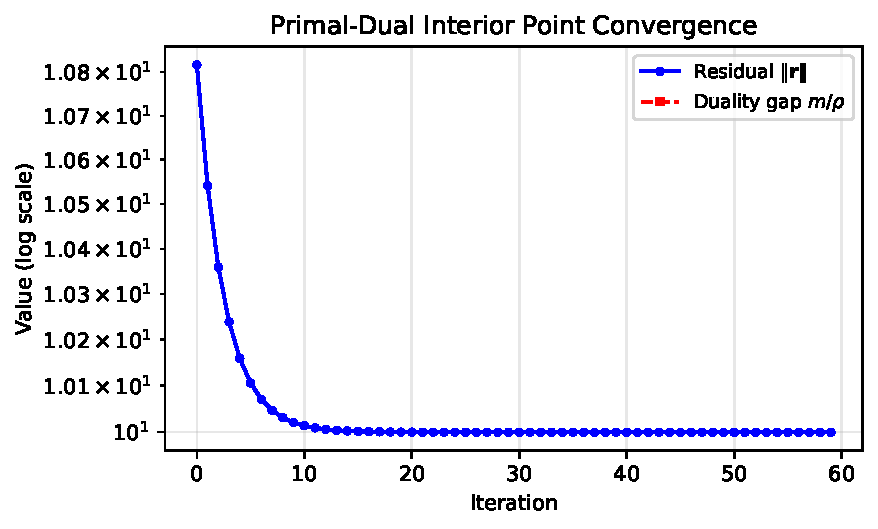
\includegraphics[width=\linewidth]{fig_primal_dual_convergence.pdf}
    \end{column}
  \end{columns}

\end{frame}

% ----
\begin{frame}[fragile]{Python: Primal-Dual Interior-Point (Algorithm 11.2)}
\begin{lstlisting}[style=python]
import numpy as np
from scipy.linalg import solve

def primal_dual_interior_point(f, gradf, hessf, gs, gradgs, hessgs,
                                rho, x, mu, alpha_max=1.0, beta=1e-4,
                                gamma=2.0, eps=0.01, p=0.9,
                                res_min=1e-4, gap_min=1e-4):
    """
    Primal-dual interior point method for:
        minimize f(x)  subject to g_i(x) <= 0  for i in 1..m
    """
    m = len(gs)
    def residual(x, mu, rho):
        r_x = gradf(x) + sum(mu[i]*gradgs[i](x) for i in range(m))
        r_mu = [-mu[i]*gs[i](x) - 1/rho for i in range(m)]
        return np.concatenate([r_x, r_mu])

    res = np.linalg.norm(residual(x, mu, rho))
    gap = sum(-mu[i]*gs[i](x) for i in range(m))

    while res > res_min or gap > gap_min:
        rho *= gamma
        # Build Jacobian and solve Newton system
        n = len(x)
        J = np.zeros((n+m, n+m))
        J[:n, :n] = hessf(x) + sum(mu[i]*hessgs[i](x) for i in range(m))
        for i in range(m):
            J[:n, n+i] = gradgs[i](x)
            J[n+i, :n] = -mu[i]*gradgs[i](x)
            J[n+i, n+i] = -gs[i](x)
        r = residual(x, mu, rho)
        d = -solve(J, r)
        d_x, d_mu = d[:n], d[n:]

        # Step size: keep mu > 0
        alpha = alpha_max
        for i in range(m):
            if d_mu[i] < 0:
                alpha = min(alpha, -(1-eps)*mu[i]/d_mu[i])

        # Keep g(x) <= 0
        while any(gs[i](x + alpha*d_x) > 0 for i in range(m)):
            alpha *= p

        # Armijo condition
        while np.linalg.norm(residual(x+alpha*d_x, mu+alpha*d_mu, rho)) \
              > (1 - beta*alpha)*res:
            alpha *= p

        x = x + alpha*d_x
        mu = mu + alpha*d_mu
        res = np.linalg.norm(residual(x, mu, rho))
        gap = sum(-mu[i]*gs[i](x) for i in range(m))

    return x, mu
\end{lstlisting}
\end{frame}

% ============================================================
\section{11.3 Dual Ascent}
% ============================================================

\begin{frame}[allowframebreaks]{Dual Ascent: Alternating Optimisation}

  Dual ascent is an iterative method that alternates between minimising
  the Lagrangian over the primal variables $\bx$ and ascending (maximising)
  the dual function over the multipliers $\bmu$ and $\blam$ (lambda).
  Because the dual function is concave, gradient ascent on it converges to
  the global maximum --- the dual optimal solution.

  \medskip
  \textbf{Why does this work?}  When strong duality holds, the optimal
  triple $(\bx^*, \bmu^*, \blam^*)$ is a saddle point of the Lagrangian:
  \[
    \calL(\bx^*, \bmu^*, \blam^*) \;=\; \min_{\bx}\, \calL(\bx, \bmu^*, \blam^*)
    \quad \text{and} \quad
    \calL(\bx^*, \bmu^*, \blam^*) \;=\; \max_{\bmu \ge \mathbf{0},\, \blam}
    \calL(\bx^*, \bmu, \blam)
  \]
  At this saddle point, no change to $\bx$ can decrease the Lagrangian, and
  no change to the multipliers can increase it.  Alternating between the two
  optimisations converges to this point.

  \begin{block}{Dual Ascent Algorithm}
    \textbf{Step 1 --- Primal update} (minimise Lagrangian over $\bx$):
    \[
      \bx^{(k+1)} \;=\; \arg\min_{\bx}\; \calL\!\left(\bx,\, \bmu^{(k)},\, \blam^{(k)}\right)
    \]
    This is an unconstrained minimisation (no constraints on $\bx$), which
    is generally easier to solve than the original constrained problem.

    \medskip
    \textbf{Step 2 --- Dual update} (gradient ascent on dual variables):
    \[
      \bmu^{(k+1)} \;=\; \max\!\left(\mathbf{0},\;\; \bmu^{(k)} + \alpha\, \bg\!\left(\bx^{(k+1)}\right)\right)
    \]
    \[
      \blam^{(k+1)} \;=\; \blam^{(k)} + \alpha\, \bh\!\left(\bx^{(k+1)}\right)
    \]
  \end{block}

  \begin{block}{Notation}
    \begin{itemize}
      \item $\bx^{(k)}$ (x superscript k): the value of $\bx$ at iteration
            number $k$.  Superscript $k$ is a counter, not a power.
      \item $\alpha$ (alpha, pronounced ``al-fa''): the step size, i.e.\
            how far we move along the gradient direction.  A larger $\alpha$
            means bigger steps; too large causes divergence.
      \item $\bg(\bx^{(k+1)})$: the vector of constraint violations at the
            new primal point.  This is the gradient of the dual function
            $\calD$ with respect to $\bmu$ --- ascent on $\calD$ means
            stepping toward positive constraint violations.
      \item $\max(\mathbf{0}, \cdot)$: the component-wise maximum with
            zero, which projects $\bmu$ onto the non-negative orthant and
            ensures $\bmu \ge \mathbf{0}$ is maintained.
    \end{itemize}
  \end{block}

  \begin{alertblock}{How to Read This}
    The dual update for $\bmu$ says: if the constraint $g_i(\bx) > 0$ is
    violated at the new primal point, increase $\mu_i$ (make the penalty
    for violating this constraint bigger).  If $g_i(\bx) < 0$ (constraint
    is satisfied with slack), decrease $\mu_i$ toward zero.  Over many
    iterations, $\mu_i$ settles at the value that perfectly prices the
    constraint.  One drawback is that dual ascent can be slow when the
    problem is ill-conditioned, because it zig-zags in the dual space.
  \end{alertblock}

\end{frame}

% ----
\begin{frame}[allowframebreaks]{Dual Ascent: Numerical Example}

  \begin{columns}
    \begin{column}{0.52\textwidth}
      \textbf{The problem:} minimise $x_1^2 + x_2^2$ subject to
      $x_1 + x_2 = 1$.  The objective is the squared distance from the
      origin; the constraint forces the solution to lie on the line
      $x_1 + x_2 = 1$.

      \medskip
      \textbf{Deriving the dual function:} the Lagrangian is
      $\calL = x_1^2 + x_2^2 + \lambda(x_1 + x_2 - 1)$.
      Setting $\partial\calL/\partial x_1 = 2x_1 + \lambda = 0$ and
      $\partial\calL/\partial x_2 = 2x_2 + \lambda = 0$ gives
      $x_1 = x_2 = -\lambda/2$.  Substituting back:

      \begin{block}{Dual Function}
        \[
          \calD(\lambda) \;=\; -\frac{\lambda^2}{2} - \lambda
        \]
      \end{block}

      Setting $\calD'(\lambda) = -\lambda - 1 = 0$ gives $\lambda^* = -1$
      and $\calD(-1) = -1/2 + 1 = 1/2 = p^*$.  Strong duality holds.

      \medskip
      \textbf{Dual ascent update rules:}
      \[
        x_i^{(k+1)} \;=\; -\lambda^{(k)} / 2
      \]
      \[
        \lambda^{(k+1)} \;=\; \lambda^{(k)} + \alpha\,
        \underbrace{(x_1 + x_2 - 1)}_{\text{constraint violation}}
      \]
    \end{column}
    \begin{column}{0.46\textwidth}
      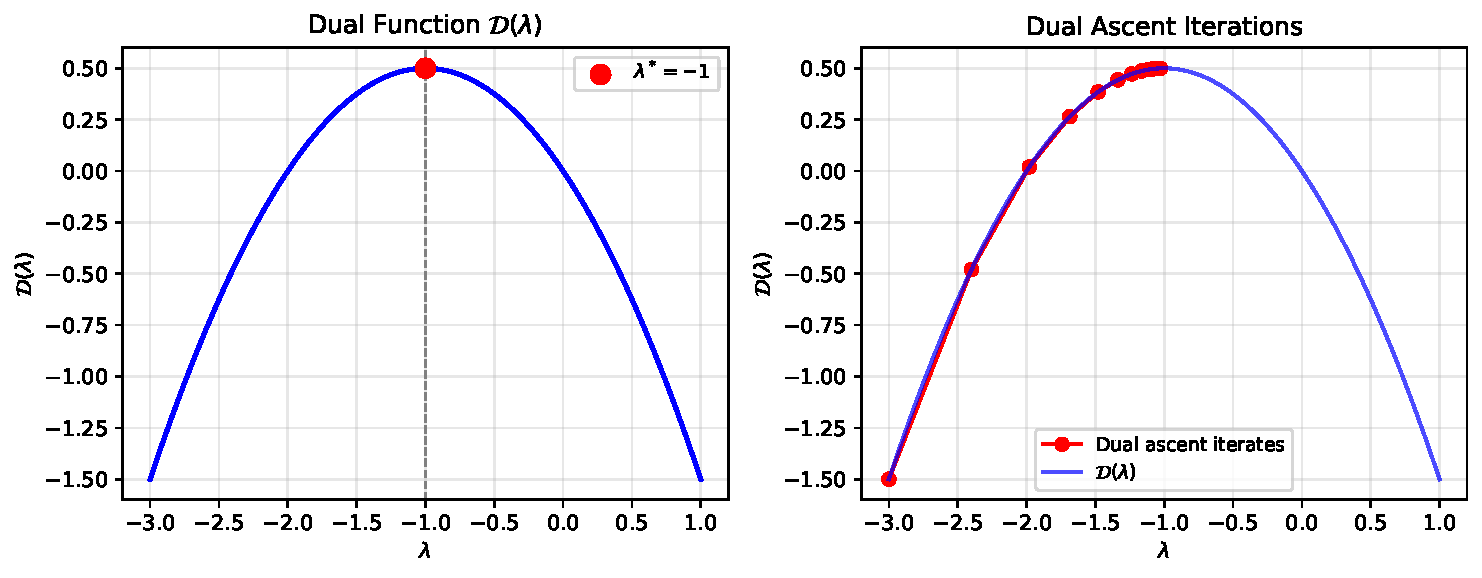
\includegraphics[width=\linewidth]{fig_dual_ascent.pdf}
    \end{column}
  \end{columns}

  \begin{exampleblock}{Worked Example: two steps with $\alpha = 0.5$}
    Start at $\lambda^{(0)} = 0$.
    \begin{itemize}
      \item Primal step: $x_1 = x_2 = -0/2 = 0$.
            Violation: $0 + 0 - 1 = -1$.
      \item Dual step: $\lambda^{(1)} = 0 + 0.5(-1) = -0.5$.
      \item Primal step: $x_1 = x_2 = -(-0.5)/2 = 0.25$.
            Violation: $0.25 + 0.25 - 1 = -0.5$.
      \item Dual step: $\lambda^{(2)} = -0.5 + 0.5(-0.5) = -0.75$.
    \end{itemize}
    The sequence converges toward $\lambda^* = -1$,
    $x_1^* = x_2^* = 1/2$.
  \end{exampleblock}

\end{frame}

% ----
\begin{frame}[allowframebreaks]{Method of Multipliers (Augmented Lagrangian)}

  Plain dual ascent can be slow, especially when the dual function is nearly
  flat (ill-conditioned problem).  The \textbf{method of multipliers} fixes
  this by adding a quadratic penalty term directly to the Lagrangian, which
  sharpens the curvature and accelerates convergence --- without requiring
  $\rho \to \infty$ as in the pure penalty method.

  \begin{block}{Augmented Lagrangian}
    \[
      \calL_\rho(\bx, \blam) \;=\;
      f(\bx) \;+\; \blam^\top \bh(\bx) \;+\;
      \frac{\rho}{2}\,\|\bh(\bx)\|_2^2
    \]
  \end{block}

  \begin{block}{Notation}
    \begin{itemize}
      \item $\calL_\rho$ (script L sub rho): the \emph{augmented} Lagrangian,
            which includes both the standard Lagrange multiplier term and a
            quadratic penalty.
      \item $\blam^\top \bh(\bx)$: the standard Lagrange multiplier term.
            $\blam^\top$ (lambda transposed) is the row vector of equality
            multipliers; multiplying by the column vector $\bh(\bx)$ gives
            the scalar dot product $\sum_j \lambda_j h_j(\bx)$.
      \item $\|\bh(\bx)\|_2^2 = \sum_j h_j(\bx)^2$: the squared Euclidean
            norm (denoted $\|\cdot\|_2^2$, ``2-norm squared'') of the
            constraint vector.  This is zero only when all equality
            constraints are satisfied.
      \item $\rho/2$: the penalty weight.  A larger $\rho$ penalises
            constraint violation more severely.
    \end{itemize}
  \end{block}

  \begin{block}{Method of Multipliers Updates}
    \[
      \bx^{(k+1)} \;=\; \arg\min_{\bx}\; \calL_\rho\!\left(\bx,\, \blam^{(k)}\right)
    \]
    \[
      \blam^{(k+1)} \;=\; \blam^{(k)} \;+\; \rho\, \bh\!\left(\bx^{(k+1)}\right)
    \]
  \end{block}

  \begin{columns}
    \begin{column}{0.54\textwidth}
      Compared to plain dual ascent (step size $\alpha$), the method of
      multipliers uses the natural step size $\rho$ for the dual update,
      and the augmented Lagrangian has stronger curvature in the primal
      direction.  This means convergence holds for any fixed $\rho > 0$
      (unlike the pure penalty method, which needs $\rho \to \infty$
      to approach feasibility).

      \medskip
      One drawback: the primal update
      $\min_\bx \calL_\rho(\bx, \blam^{(k)})$ must be solved jointly
      over all components of $\bx$, which prevents easy parallelisation.
      ADMM (the next section) addresses this limitation.
    \end{column}
    \begin{column}{0.44\textwidth}
      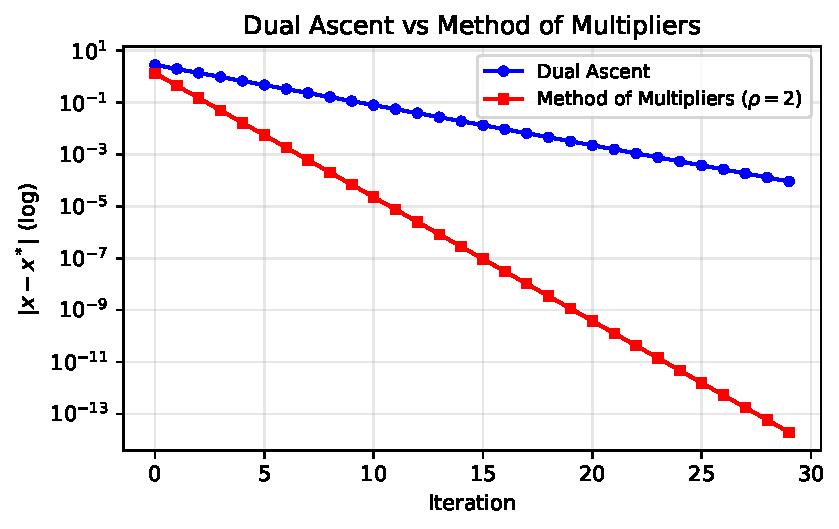
\includegraphics[width=\linewidth]{fig_method_of_multipliers.pdf}
    \end{column}
  \end{columns}

\end{frame}

% ============================================================
\section{11.4 ADMM}
% ============================================================

\begin{frame}[allowframebreaks]{ADMM: Alternating Direction Method of Multipliers}

  ADMM combines the benefits of dual ascent (decomposability) and the
  method of multipliers (convergence for fixed $\rho$).  It does so by
  splitting the problem into two separate sub-problems that can each be
  solved independently, then combining results via a shared multiplier.

  The problem must be written in the following \textbf{canonical ADMM form}:

  \begin{block}{ADMM Canonical Form}
    \[
      \min_{\bx_1, \bx_2}\; f_1(\bx_1) + f_2(\bx_2)
      \quad \text{subject to} \quad
      \bA_1 \bx_1 + \bA_2 \bx_2 = \bb
    \]
  \end{block}

  \begin{block}{Notation}
    \begin{itemize}
      \item $\bx_1 \in \R^{n_1}$, $\bx_2 \in \R^{n_2}$: the two blocks of
            primal variables.  Splitting into two blocks is what enables
            alternating optimisation.
      \item $f_1, f_2$: two convex objective functions, one for each block.
            They need not have the same form.
      \item $\bA_1 \in \R^{p \times n_1}$, $\bA_2 \in \R^{p \times n_2}$:
            matrices (capital bold A) that couple the two blocks in the
            linear equality constraint.
      \item $\bb \in \R^p$: the right-hand side (bold lowercase b) of the
            coupling equality.
    \end{itemize}
  \end{block}

  \framebreak

  \textbf{Augmented Lagrangian for ADMM:}
  \[
    \calL_\rho(\bx_1, \bx_2, \blam)
    \;=\; f_1(\bx_1) + f_2(\bx_2)
    \;+\; \blam^\top(\bA_1\bx_1 + \bA_2\bx_2 - \bb)
    \;+\; \frac{\rho}{2}\,\|\bA_1\bx_1 + \bA_2\bx_2 - \bb\|_2^2
  \]

  \begin{block}{ADMM Updates}
    \begin{align*}
      \bx_1^{(k+1)} &\;=\; \arg\min_{\bx_1}\;
        \calL_\rho\!\left(\bx_1,\, \bx_2^{(k)},\, \blam^{(k)}\right)
        \quad \textit{(update $\bx_1$, fix $\bx_2$)}\\[4pt]
      \bx_2^{(k+1)} &\;=\; \arg\min_{\bx_2}\;
        \calL_\rho\!\left(\bx_1^{(k+1)},\, \bx_2,\, \blam^{(k)}\right)
        \quad \textit{(update $\bx_2$, fix new $\bx_1$)}\\[4pt]
      \blam^{(k+1)} &\;=\; \blam^{(k)}
        \;+\; \rho\!\left(\bA_1\bx_1^{(k+1)} + \bA_2\bx_2^{(k+1)} - \bb\right)
        \quad \textit{(dual update)}
    \end{align*}
  \end{block}

  The \emph{alternating direction} is the key feature: rather than
  minimising jointly over $(\bx_1, \bx_2)$ together (which may be
  expensive), we alternate between the two sub-problems.  Each sub-problem
  is typically much cheaper to solve.  After updating $\bx_1$ and $\bx_2$,
  the dual variable $\blam$ is updated using the constraint violation
  $\bA_1\bx_1 + \bA_2\bx_2 - \bb$, which is the gradient of the
  augmented Lagrangian with respect to $\blam$.

\end{frame}

% ----
\begin{frame}[allowframebreaks]{ADMM Block Diagram and Convergence}

  \begin{columns}
    \begin{column}{0.50\textwidth}
      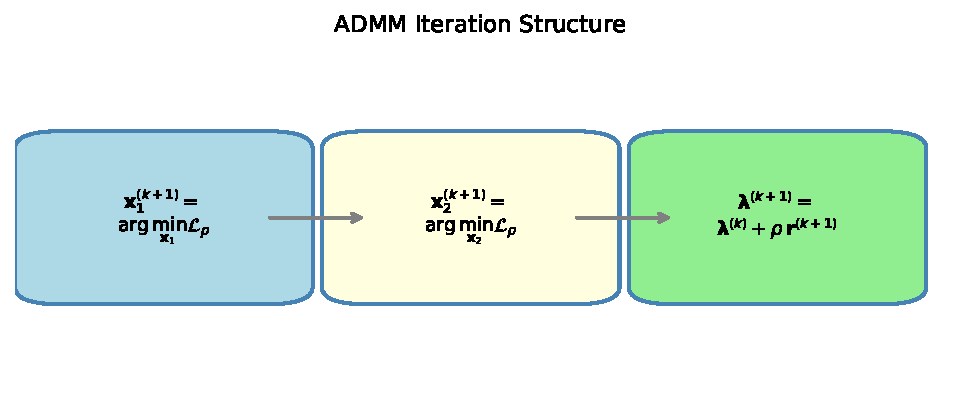
\includegraphics[width=\linewidth]{fig_admm_block.pdf}

      \medskip
      \textbf{Stopping criteria:} we monitor two residuals to decide
      when ADMM has converged.

      \begin{block}{Primal Residual $\mathbf{r}^{(k+1)}$}
        \[
          \mathbf{r}^{(k+1)}
          \;=\; \bA_1\bx_1^{(k+1)} + \bA_2\bx_2^{(k+1)} - \bb
        \]
        This measures how well the coupling constraint
        $\bA_1\bx_1 + \bA_2\bx_2 = \bb$ is satisfied.
      \end{block}

      \begin{block}{Dual Residual $\mathbf{s}^{(k+1)}$}
        \[
          \mathbf{s}^{(k+1)}
          \;=\; \rho\, \bA_2^\top\!\left(\bx_2^{(k+1)} - \bx_2^{(k)}\right)
        \]
        This measures stationarity of the Lagrangian with respect to
        $\bx_2$ --- it is large when $\bx_2$ is still changing rapidly.
      \end{block}

      Stop when $\|\mathbf{r}\| < \varepsilon_r$ (epsilon sub r) and
      $\|\mathbf{s}\| < \varepsilon_s$ (epsilon sub s), where
      $\varepsilon_r, \varepsilon_s > 0$ are prescribed tolerances.
    \end{column}
    \begin{column}{0.48\textwidth}
      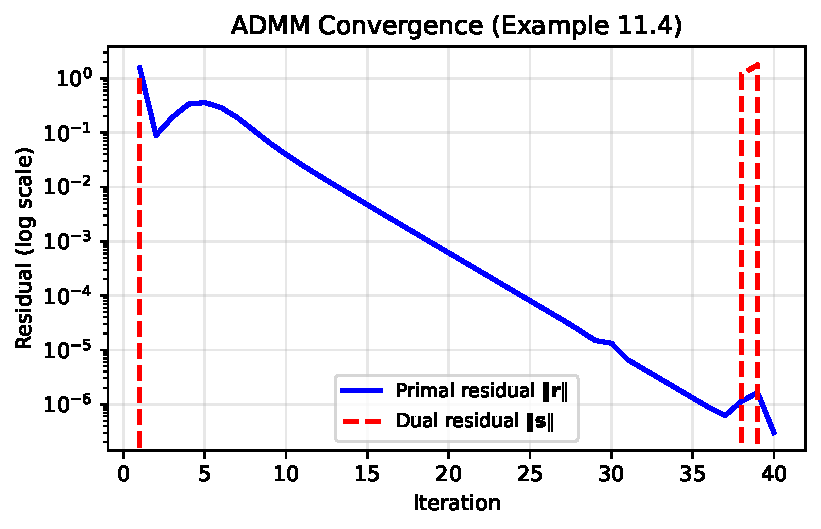
\includegraphics[width=\linewidth]{fig_admm_convergence.pdf}

      \medskip
      \textbf{Adaptive $\rho$:} the penalty parameter $\rho$ (rho) can be
      adjusted during the run to balance primal and dual convergence:
      \begin{itemize}
        \item If $\|\mathbf{r}\| \gg \|\mathbf{s}\|$ (primal residual much
              larger than dual), \textbf{increase} $\rho$.  This pushes
              the iterates toward primal feasibility more aggressively.
        \item If $\|\mathbf{s}\| \gg \|\mathbf{r}\|$ (dual residual much
              larger), \textbf{decrease} $\rho$.  This gives the dual
              variable more room to move.
        \item Self-adaptive $\rho$ can significantly improve convergence
              in practice without tuning by hand.
      \end{itemize}
    \end{column}
  \end{columns}

\end{frame}

% ----
\begin{frame}[allowframebreaks]{Scaled ADMM Form}

  It is often convenient to rescale the dual variable $\blam$ by dividing
  by $\rho$, defining a \textbf{scaled dual variable}:
  \[
    \bu \;=\; \frac{1}{\rho}\,\blam
  \]
  Here $\bu$ (bold u) is called the scaled dual variable.  This
  simplifies the update formulas considerably.

  \medskip
  Substituting $\blam = \rho\,\bu$ into the augmented Lagrangian,
  completing the square, and dropping constant terms gives:
  \[
    \calL_\rho(\bx_1, \bx_2, \blam)
    \;=\; f_1(\bx_1) + f_2(\bx_2)
    + \frac{\rho}{2}\,\|\bA_1\bx_1 + \bA_2\bx_2 - \bb + \bu\|_2^2
    - \frac{\rho}{2}\,\|\bu\|_2^2
  \]

  \begin{block}{Scaled ADMM Updates}
    \[
      \bx_1^{(k+1)} \;=\; \arg\min_{\bx_1}\;
        f_1(\bx_1) + \frac{\rho}{2}\,\|\bA_1\bx_1 - \bv^{(k)}\|_2^2,
      \quad \bv^{(k)} = -\bA_2\bx_2^{(k)} + \bb - \bu^{(k)}
    \]
    \[
      \bx_2^{(k+1)} \;=\; \arg\min_{\bx_2}\;
        f_2(\bx_2) + \frac{\rho}{2}\,\|\bA_2\bx_2 - \bw^{(k)}\|_2^2,
      \quad \bw^{(k)} = -\bA_1\bx_1^{(k+1)} + \bb - \bu^{(k)}
    \]
    \[
      \bu^{(k+1)} \;=\; \bu^{(k)} + \bA_1\bx_1^{(k+1)} + \bA_2\bx_2^{(k+1)} - \bb
      \;=\; \bu^{(0)} + \sum_{j=1}^{k+1} \mathbf{r}^{(j)}
    \]
  \end{block}

  \begin{block}{Notation}
    \begin{itemize}
      \item $\bv^{(k)}$, $\bw^{(k)}$: auxiliary target vectors that
            consolidate the current values of the other block and the
            scaled dual variable into a single ``target'' that $\bx_1$
            (or $\bx_2$) is being pulled toward.
      \item The scaled dual update $\bu^{(k+1)} = \bu^{(k)} + \mathbf{r}^{(k+1)}$
            is simply the \textbf{running sum of all past primal residuals}
            $\mathbf{r}^{(j)} = \bA_1\bx_1^{(j)} + \bA_2\bx_2^{(j)} - \bb$.
    \end{itemize}
  \end{block}

  \begin{alertblock}{Key Insight}
    Each sub-problem for $\bx_1$ and $\bx_2$ now has the form:
    minimise $f_i(\bx_i) + \frac{\rho}{2}\|\bA_i\bx_i - \text{target}\|_2^2$.
    This is a \emph{proximal minimisation} of $f_i$ with a quadratic
    proximity term pulling toward the target.  Many standard functions
    (e.g.\ $\ell_1$ norm, indicator of a convex set) have closed-form
    proximal operators, making each ADMM step very efficient.
  \end{alertblock}

\end{frame}

% ----
\begin{frame}[fragile]{Python: ADMM Core Implementation}
\begin{lstlisting}[style=python]
import numpy as np

def admm(f1_prox, f2_prox, A1, A2, b, rho=1.0, gamma=1.5,
         eps_r=1e-3, eps_s=1e-3, max_iter=200):
    """
    ADMM solver for:  min f1(x1) + f2(x2)  s.t.  A1@x1 + A2@x2 = b

    f1_prox(v, rho):  proximal operator of f1 -- argmin f1(x)+rho/2||x-v||^2
    f2_prox(v, rho):  proximal operator of f2
    """
    n1 = A1.shape[1]; n2 = A2.shape[1]
    x1 = np.zeros(n1); x2 = np.zeros(n2); u = np.zeros(len(b))

    for k in range(max_iter):
        # x1-update: minimise f1(x1) + rho/2 ||A1 x1 - v||^2
        v = -A2 @ x2 + b - u
        x1 = f1_prox(A1, v, rho)      # application-specific solver

        # x2-update: minimise f2(x2) + rho/2 ||A2 x2 - w||^2
        w = -A1 @ x1 + b - u
        x2 = f2_prox(A2, w, rho)

        # dual (scaled) variable update
        r = A1 @ x1 + A2 @ x2 - b    # primal residual
        s = rho * A1.T @ (x2 - x2)   # dual residual (simplified)
        u = u + r

        if np.linalg.norm(r) < eps_r and np.linalg.norm(s) < eps_s:
            print(f"ADMM converged at iteration {k+1}")
            break

        # Adaptive rho (Boyd et al. 2011)
        if np.linalg.norm(r) > 10 * np.linalg.norm(s):
            rho *= gamma
        elif np.linalg.norm(s) > 10 * np.linalg.norm(r):
            rho /= gamma

    return x1, x2
\end{lstlisting}
\end{frame}

% ============================================================
\section{11.5 ADMM Applications}
% ============================================================

\begin{frame}[allowframebreaks]{11.5.1 General Constrained Optimisation in ADMM Form}

  Any constrained optimisation problem can be reformulated in the ADMM
  canonical form by introducing an auxiliary variable $\bx_2$ and using
  the \emph{indicator function} of the feasible set as one of the
  objective terms.

  \medskip
  \textbf{Reformulation:} given $\min_\bx f(\bx)$ subject to
  $\bx \in \mathcal{X}$ (calligraphic X, some convex constraint set),
  we write:
  \[
    \min_{\bx_1,\, \bx_2}\;
    \underbrace{f(\bx_1)}_{f_1}
    + \underbrace{\mathbb{1}_{\mathcal{X}}(\bx_2)}_{f_2}
    \quad \text{subject to} \quad \bx_1 - \bx_2 = \mathbf{0}
  \]
  where $\mathbb{1}_{\mathcal{X}}(\bx_2) = 0$ if $\bx_2 \in \mathcal{X}$,
  and $+\infty$ otherwise.  This indicator function encodes the constraint:
  any solution with $\bx_2 \notin \mathcal{X}$ has infinite cost.

  \begin{block}{Proximal Minimisation}
    Each ADMM sub-problem has the form:
    \[
      \arg\min_{\bx}\; f(\bx) + \frac{\rho}{2}\,\|\bx - \bp\|_2^2
    \]
    where $\bp$ (bold p) is the current ``target'' point.  If $f$ is
    differentiable, a first-order approximation gives the gradient step:
    \[
      \bx \;\approx\; \bp - \frac{1}{\rho}\,\grad f(\bp)
    \]
    This says: start at $\bp$, then take a step of size $1/\rho$ in the
    direction of steepest descent of $f$.
  \end{block}

  The $\bx_2$-sub-problem with $f_2 = \mathbb{1}_{\mathcal{X}}$ has an
  especially simple solution: it is the \textbf{projection} of the current
  $\bx_1 + \bu$ onto the set $\mathcal{X}$, denoted
  $\text{proj}_{\mathcal{X}}(\bx_1^{(k+1)} + \bu^{(k)})$.  Projection
  operators onto common sets (boxes, cones, affine subspaces) often have
  closed-form expressions.

\end{frame}

% ----
\begin{frame}[allowframebreaks]{11.5.2 Alternating Projections}

  \textbf{Goal:} find a point $\bx$ that belongs to the intersection of
  two convex sets, $\bx \in \mathcal{X}_1 \cap \mathcal{X}_2$.  This arises
  in image reconstruction, signal processing, and constraint satisfaction.

  \medskip
  \textbf{ADMM formulation:}
  \[
    \min_{\bx_1,\, \bx_2}\;
    \mathbb{1}_{\mathcal{X}_1}(\bx_1) + \mathbb{1}_{\mathcal{X}_2}(\bx_2)
    \quad \text{subject to} \quad \bx_1 - \bx_2 = \mathbf{0}
  \]
  Both sub-problems are projections: the $\bx_1$-update projects onto
  $\mathcal{X}_1$, and the $\bx_2$-update projects onto $\mathcal{X}_2$.

  \begin{columns}
    \begin{column}{0.52\textwidth}
      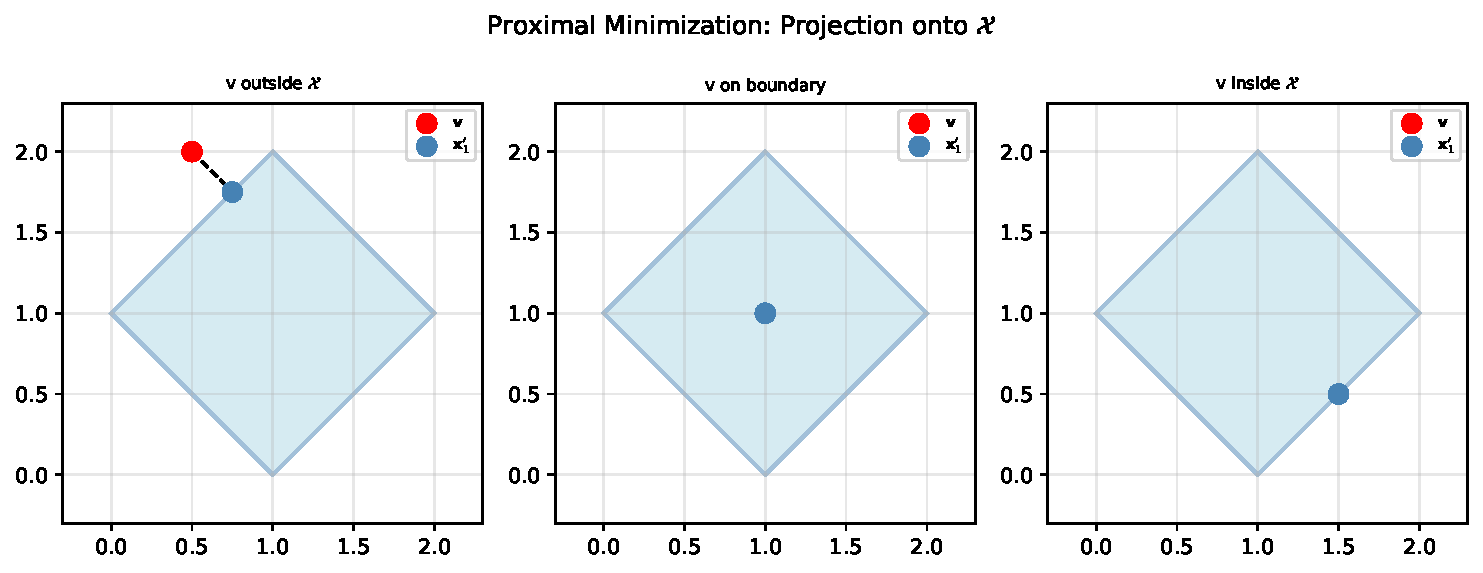
\includegraphics[width=\linewidth]{fig_proximal.pdf}
    \end{column}
    \begin{column}{0.46\textwidth}
      \textbf{Von Neumann's alternating projections algorithm} simply
      bounces between the two sets: project onto $\mathcal{X}_1$, then
      onto $\mathcal{X}_2$, and repeat.  This converges to the
      intersection but can be very slow when the two sets meet at a
      narrow angle (like the inside of a thin wedge).

      \medskip
      \textbf{Dykstra's algorithm} (which is equivalent to ADMM here)
      introduces a correction term $\bu$ at each step.  This correction
      acts like a momentum term that remembers the accumulated constraint
      violations and steers the iterates more directly toward the
      intersection.  Dykstra converges significantly faster than Von
      Neumann in difficult geometries.
    \end{column}
  \end{columns}

\end{frame}

% ----
\begin{frame}[allowframebreaks]{11.5.3 Least Absolute Deviations (LAD)}

  Ordinary least squares minimises $\|\bA\bx - \bb\|_2^2$, which is
  sensitive to outliers because large errors are squared.  \textbf{Least
  Absolute Deviations (LAD)} instead minimises $\|\bA\bx - \bb\|_1$
  (the sum of absolute residuals), which is much more robust.

  \begin{block}{LAD Problem}
    \[
      \min_{\bx}\; \|\bA\bx - \bb\|_1
      \;=\; \sum_{i=1}^m |(\bA\bx - \bb)_i|
    \]
  \end{block}

  \textbf{ADMM formulation:} introduce $\bx_2 = \bA\bx_1 - \bb$:
  \[
    \min_{\bx_1,\, \bx_2}\; f_1(\bx_1) + \|\bx_2\|_1
    \quad \text{subject to} \quad \bA\bx_1 - \bx_2 = \bb
  \]

  The key to solving the $\bx_2$-update is the \textbf{soft thresholding
  operator}, which is the proximal operator of the $\ell_1$ (L1) norm:

  \begin{block}{Soft Thresholding Operator $S_\kappa$}
    \[
      (S_\kappa(\bx))_i \;=\;
      \begin{cases}
        x_i + \kappa & x_i < -\kappa \\
        0            & |x_i| \le \kappa \\
        x_i - \kappa & x_i > \kappa
      \end{cases}
      \;=\; \operatorname{sign}(x_i)\,\max(|x_i| - \kappa,\; 0)
    \]
  \end{block}

  \begin{block}{Notation}
    \begin{itemize}
      \item $\kappa$ (kappa, pronounced ``cap-a''): the threshold level.
            Values of $|x_i|$ smaller than $\kappa$ are shrunk to exactly
            zero; larger values are shifted toward zero by $\kappa$.
      \item $\operatorname{sign}(x_i)$: returns $+1$ if $x_i > 0$,
            $-1$ if $x_i < 0$, and $0$ if $x_i = 0$.
    \end{itemize}
  \end{block}

  \begin{alertblock}{How to Read This}
    Soft thresholding shrinks every element of a vector toward zero by
    the amount $\kappa$, and sets it to exactly zero if it was already
    smaller than $\kappa$ in magnitude.  It is the ``soft'' version of
    hard thresholding (which would set small values to zero and leave
    large values unchanged).  Soft thresholding is the key operation
    that produces sparse solutions.
  \end{alertblock}

  \begin{columns}
    \begin{column}{0.40\textwidth}
      \textbf{LAD ADMM updates:}
      \begin{align*}
        \bx_1' &= (\bA^\top\bA)^{-1}\bA^\top(\bb + \bx_2 - \bu) \\
        \bx_2' &= S_{1/\rho}(\bA\bx_1' - \bb + \bu) \\
        \bu'   &= \bu + \bA\bx_1' - \bb - \bx_2'
      \end{align*}
      The Cholesky factorisation of $\bA^\top\bA$ is precomputed once,
      making each iteration $O(mn)$ instead of $O(n^3)$.
    \end{column}
    \begin{column}{0.58\textwidth}
      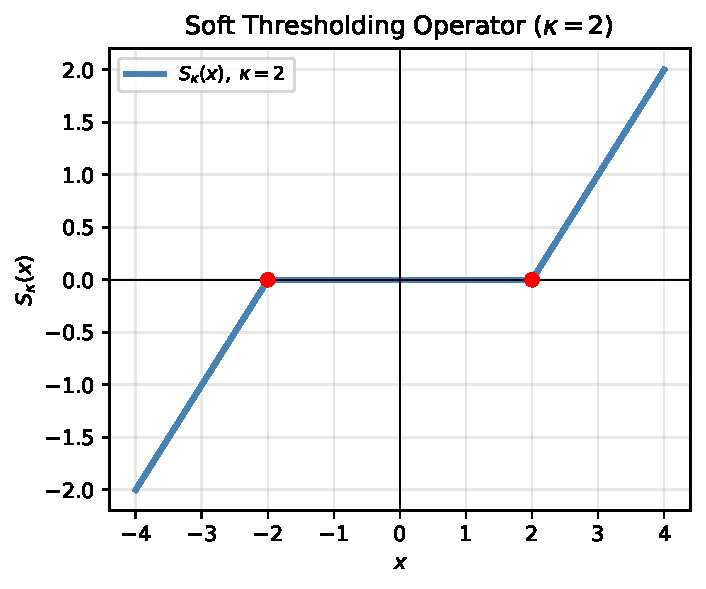
\includegraphics[width=\linewidth]{fig_soft_threshold.pdf}
    \end{column}
  \end{columns}

\end{frame}

% ----
\begin{frame}[allowframebreaks]{11.5.4 Basis Pursuit (Split Bregman)}

  \textbf{Basis pursuit} finds the sparsest solution to an underdetermined
  linear system.  In compressed sensing and signal recovery, we observe
  a short measurement vector $\bb$ and know a measurement matrix $\bA$,
  and we want to recover a high-dimensional sparse signal $\bx$:

  \begin{block}{Basis Pursuit Problem}
    \[
      \min_{\bx}\; \|\bx\|_1
      \quad \text{subject to} \quad
      \bA\bx = \bb
    \]
  \end{block}

  The $\ell_1$ norm $\|\bx\|_1 = \sum_i |x_i|$ promotes sparsity: solutions
  with many zero components are preferred because they have smaller
  $\ell_1$ norm (for the same constraint satisfaction) than dense solutions.

  \medskip
  \textbf{ADMM reformulation:} split $\bx$ into two copies $\bx_1 = \bx_2$,
  putting the $\ell_1$ penalty on $\bx_2$ and the equality constraint on
  $\bx_1$:

  \begin{block}{ADMM Updates for Basis Pursuit}
    \[
      \bx_1' \;=\;
      \bigl(\bI - \bA^\top(\bA\bA^\top)^{-1}\bA\bigr)(\bx_2 - \bu)
      + \bA^\top(\bA\bA^\top)^{-1}\bb
    \]
    \[
      \bx_2' \;=\; S_{1/\rho}(\bx_1' + \bu)
      \qquad
      \bu' \;=\; \bu + \bx_1' - \bx_2'
    \]
  \end{block}

  \begin{block}{Notation}
    \begin{itemize}
      \item $\bI - \bA^\top(\bA\bA^\top)^{-1}\bA$: the
            \emph{orthogonal projector} onto the null space of $\bA$
            (the set of all $\bx$ satisfying $\bA\bx = \mathbf{0}$).
      \item $\bA^\top(\bA\bA^\top)^{-1}\bb$: the minimum-norm particular
            solution to $\bA\bx = \bb$ (the pseudo-inverse solution).
      \item The $\bx_1'$ update therefore takes any starting point
            $\bx_2 - \bu$, projects it onto the feasible affine subspace
            $\{\bx : \bA\bx = \bb\}$.
    \end{itemize}
  \end{block}

  Both matrices $\bI - \bA^\top(\bA\bA^\top)^{-1}\bA$ and
  $\bA^\top(\bA\bA^\top)^{-1}\bb$ can be precomputed once (costing
  $O(p^3)$ for the matrix inverse of the $p \times p$ Gram matrix
  $\bA\bA^\top$).  Each subsequent iteration then costs only one
  matrix-vector product ($O(np)$) plus soft thresholding ($O(n)$).
  This method is also known as the \textbf{split Bregman} method.

\end{frame}

% ----
\begin{frame}[allowframebreaks]{11.5.5 Lasso: $L_1$-Regularised Regression}

  \begin{columns}
    \begin{column}{0.55\textwidth}
      \textbf{The Lasso} (Least Absolute Shrinkage and Selection Operator)
      balances fitting a linear model to data against producing a sparse
      coefficient vector:

      \begin{block}{Lasso Problem}
        \[
          \min_{\bx}\;
          \frac{1}{2}\,\|\bA\bx - \bb\|_2^2
          \;+\; \lambda\,\|\bx\|_1
        \]
      \end{block}

      \begin{block}{Notation}
        \begin{itemize}
          \item $\frac{1}{2}\|\bA\bx - \bb\|_2^2$: the least-squares
                fit term, measuring how well $\bA\bx$ approximates $\bb$.
                The factor $1/2$ is included for convenience so the
                gradient equals $\bA^\top(\bA\bx - \bb)$ without a
                factor of 2.
          \item $\lambda\,\|\bx\|_1$ (lambda times L1 norm): the
                regularisation term.  $\lambda \ge 0$ (lambda, ``lam-da'')
                controls the sparsity trade-off.  Larger $\lambda$ pushes
                more coefficients to exactly zero.
        \end{itemize}
      \end{block}

      \textbf{ADMM formulation:} $f_1(\bx_1) = \frac{1}{2}\|\bA\bx_1 - \bb\|_2^2$,
      $f_2(\bx_2) = \lambda\|\bx_2\|_1$, subject to $\bx_1 - \bx_2 = \mathbf{0}$.
    \end{column}
    \begin{column}{0.43\textwidth}
      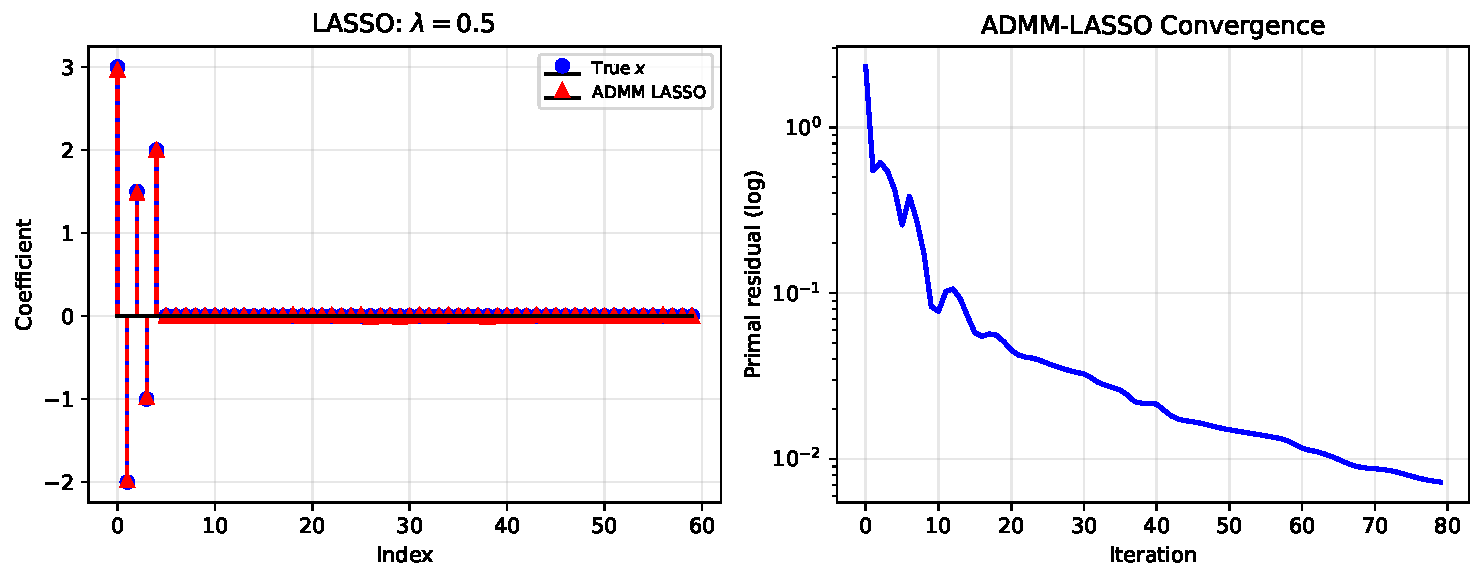
\includegraphics[width=\linewidth]{fig_lasso.pdf}
    \end{column}
  \end{columns}

  \begin{block}{Lasso ADMM Updates}
    \[
      \bx_1' \;=\; (\bA^\top\bA + \rho\bI)^{-1}
      \bigl(\bA^\top\bb + \rho(\bx_2 - \bu)\bigr)
    \]
    \[
      \bx_2' \;=\; S_{\lambda/\rho}(\bx_1' + \bu)
    \]
    \[
      \bu' \;=\; \bu + \bx_1' - \bx_2'
    \]
  \end{block}

  \begin{block}{Notation}
    \begin{itemize}
      \item $\bA^\top\bA + \rho\bI$: adding $\rho\bI$ (rho times the
            identity matrix $\bI$) to $\bA^\top\bA$ makes it strictly
            positive definite for any $\rho > 0$, guaranteeing
            invertibility even when $\bA$ is rank-deficient.
      \item $S_{\lambda/\rho}$: soft thresholding with threshold $\lambda/\rho$.
            As $\rho$ decreases, the threshold $\lambda/\rho$ increases,
            producing sparser solutions.
    \end{itemize}
  \end{block}

  The matrix $\bA^\top\bA + \rho\bI$ can be factorised (e.g.\ via
  Cholesky) once at the start, making the $\bx_1$-update a single
  triangular solve at each iteration ($O(n^2)$ after factorisation).

\end{frame}

% ----
\begin{frame}[fragile]{Python: ADMM-Lasso Implementation (Algorithm 11.7)}
\begin{lstlisting}[style=python]
import numpy as np

def lasso_admm(A, b, lam, x1=None, x2=None, rho=1.0,
               gamma=2.0, eps=1e-3, max_iter=100):
    """
    Solve  min 0.5*||Ax - b||^2 + lam*||x||_1
    via ADMM (Algorithm 11.7 in Python).
    """
    n = A.shape[1]
    if x1 is None: x1 = np.zeros(n)
    if x2 is None: x2 = np.zeros(n)
    u = np.zeros(n)

    AtA = A.T @ A
    Atb = A.T @ b

    def soft(v, kappa):
        return np.sign(v) * np.maximum(np.abs(v) - kappa, 0)

    for k in range(max_iter):
        # x1-update: linear system solve (warm-startable)
        x1 = np.linalg.solve(AtA + rho * np.eye(n),
                              Atb + rho * (x2 - u))
        # x2-update: soft thresholding
        x2 = soft(x1 + u, lam / rho)
        # scaled dual update
        u  = u + x1 - x2

        r = np.linalg.norm(x1 - x2)   # primal residual
        if r < eps:
            break
    return x1   # sparse coefficient vector

# Example usage
np.random.seed(42)
m, n = 50, 200
A = np.random.randn(m, n)
x_true = np.zeros(n); x_true[:5] = [3., -2., 1.5, -1., 2.]
b = A @ x_true + 0.1*np.random.randn(m)
x_hat = lasso_admm(A, b, lam=0.1)
print(f"Support recovery: {np.sum(np.abs(x_hat)>0.1)} nonzeros found")
\end{lstlisting}
\end{frame}

% ----
\begin{frame}[allowframebreaks]{Huber Loss and Other ADMM Applications}

  \begin{columns}
    \begin{column}{0.52\textwidth}
      The \textbf{Huber loss} is a hybrid between squared ($\ell_2$) and
      absolute ($\ell_1$) error that is both smooth near zero and robust
      to outliers far from zero:

      \begin{block}{Huber Loss}
        \[
          \operatorname{huber}(x) \;=\;
          \begin{cases}
            \tfrac{1}{2}x^2 & |x| \le 1 \\
            |x| - \tfrac{1}{2} & |x| > 1
          \end{cases}
        \]
      \end{block}

      \begin{alertblock}{How to Read This}
        For small residuals ($|x| \le 1$): the Huber loss grows
        quadratically, just like squared error, giving smooth
        gradients near the optimum.  For large residuals ($|x| > 1$):
        the loss grows only linearly, like the absolute value, so
        outliers contribute at most linearly and do not dominate
        the fit.  This makes Huber regression robust without
        sacrificing smoothness.
      \end{alertblock}

      The $\bx_2$-update for Huber regression in ADMM is:
      \[
        \bx_2' \;=\; \frac{\rho}{1+\rho}(\bA\bx_1' - \bb + \bu)
        + \frac{1}{1+\rho} S_{1+1/\rho}(\bA\bx_1' - \bb + \bu)
      \]
      This is a weighted combination of a linear term and a soft-thresholded
      term, encoding the two regimes of the Huber loss.
    \end{column}
    \begin{column}{0.46\textwidth}
      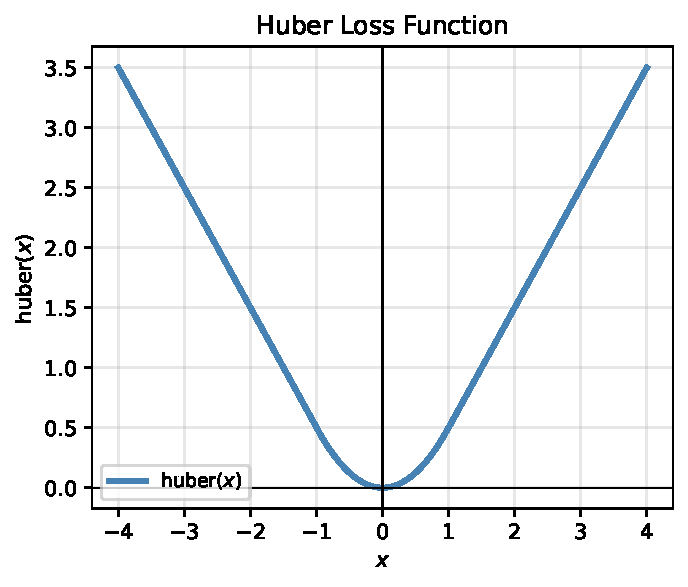
\includegraphics[width=\linewidth]{fig_huber.pdf}
    \end{column}
  \end{columns}

  \medskip
  \textbf{Summary of ADMM application patterns:}

  \begin{center}
  \renewcommand{\arraystretch}{1.2}
  \begin{tabular}{lll}
    \toprule
    Application & $f_2(\bx_2)$ & $\bx_2$-update \\
    \midrule
    Constrained opt. & $\mathbb{1}_{\mathcal{X}}$ (indicator) & Project onto $\mathcal{X}$ \\
    Basis pursuit & $\|\cdot\|_1$ ($\ell_1$ norm) & Soft threshold \\
    Lasso & $\lambda\|\cdot\|_1$ & Soft threshold (scaled) \\
    LAD regression & $\|\cdot\|_1$ & Soft threshold \\
    Huber regression & huber loss & Blend of linear + soft \\
    \bottomrule
  \end{tabular}
  \end{center}

  The pattern is always the same: one sub-problem handles the smooth
  objective (solved by a linear system), the other handles the
  non-smooth or constrained term (solved by a proximal/projection step).

\end{frame}

% ============================================================
\section{11.6 Distributed Methods}
% ============================================================

\begin{frame}[allowframebreaks]{Consensus Optimisation}

  In many large-scale problems, the objective is the sum of $k$ separate
  functions:
  \[
    \min_{\bx}\; f_1(\bx) + f_2(\bx) + \cdots + f_k(\bx)
  \]
  This arises naturally when $k$ different agents (processors, data shards,
  or physical subsystems) each have their own local objective $f_i$, but
  all must agree on a common decision variable $\bx$.  The challenge is to
  optimise the sum without collecting all data in one place.

  \medskip
  \textbf{Consensus reformulation:} introduce a local copy
  $\bx_1^{(i)}$ for each agent, and a global variable $\bx_2$ that all
  local copies must agree with:

  \begin{block}{ADMM Consensus Form}
    \[
      \min_{\bx_1^{(1)}, \ldots, \bx_1^{(k)},\; \bx_2}\;
      \sum_{i=1}^k f_i\!\left(\bx_1^{(i)}\right)
      \quad \text{subject to} \quad
      \bx_1^{(i)} = \bx_2 \quad \forall\, i = 1, \ldots, k
    \]
  \end{block}

  \begin{block}{Notation}
    \begin{itemize}
      \item $\bx_1^{(i)}$ (x sub 1 superscript i): agent $i$'s local copy
            of the decision variable.
      \item $\bx_2$: the global consensus variable that all agents must
            agree with.
      \item $\forall\, i$ (for all i): the constraint must hold for every
            agent $i = 1, \ldots, k$.
    \end{itemize}
  \end{block}

  \framebreak

  \begin{block}{Consensus ADMM Updates}
    \textbf{Step 1 --- Local updates} (all $k$ agents update in parallel):
    \[
      \bigl(\bx_1^{(i)}\bigr)' \;=\; \arg\min_{\bx_1^{(i)}}\;
      f_i\!\left(\bx_1^{(i)}\right)
      + \bigl(\blam^{(i)}\bigr)^\top\!\left(\bx_1^{(i)} - \bx_2\right)
      + \frac{\rho}{2}\,\bigl\|\bx_1^{(i)} - \bx_2\bigr\|_2^2
    \]

    \textbf{Step 2 --- Consensus update} (global averaging):
    \[
      \bx_2' \;=\; \frac{1}{k}\sum_{i=1}^k
      \left[\bigl(\bx_1^{(i)}\bigr)' + \frac{1}{\rho}\,\blam^{(i)}\right]
    \]

    \textbf{Step 3 --- Dual updates} (one per agent):
    \[
      \bigl(\blam^{(i)}\bigr)' \;=\; \blam^{(i)}
      + \rho\left[\bigl(\bx_1^{(i)}\bigr)' - \bx_2'\right]
    \]
  \end{block}

  \begin{alertblock}{Key Insight}
    Step 1 runs entirely in parallel: each agent $i$ solves its own
    sub-problem involving only $f_i$, $\blam^{(i)}$ (its own multiplier),
    and the current global consensus $\bx_2$.  The sub-problem details of
    $f_i$ do not need to be shared with anyone.  Only the local solutions
    $(\bx_1^{(i)})'$ and the multipliers $\blam^{(i)}$ need to be
    communicated to compute the average in Step 2.  This makes consensus
    ADMM suitable for \emph{federated learning} and privacy-preserving
    distributed optimisation.
  \end{alertblock}

\end{frame}

% ----
\begin{frame}[allowframebreaks]{Consensus ADMM: Convergence to Mean}

  \begin{columns}
    \begin{column}{0.52\textwidth}
      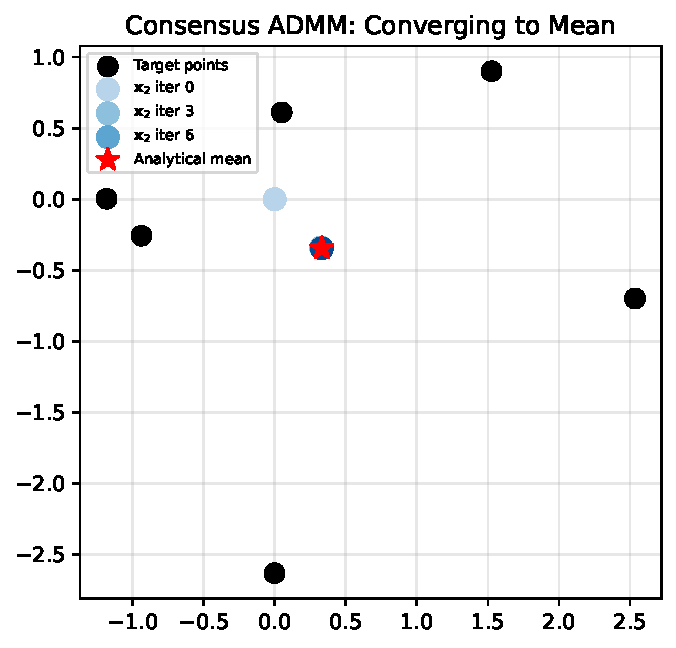
\includegraphics[width=\linewidth]{fig_consensus.pdf}
    \end{column}
    \begin{column}{0.46\textwidth}
      \textbf{How consensus ADMM converges:}

      Initially, each agent's local copy $\bx_1^{(i)}$ focuses on
      minimising its own $f_i$ without caring about the others.  This
      gives a diverse set of local optima.  The dual variables
      $\blam^{(i)}$ (lambda for agent $i$) then penalise divergence
      between $\bx_1^{(i)}$ and the global mean $\bx_2$.  Over
      successive iterations, the dual variables grow until the
      disagreement cost outweighs the individual objective savings,
      and all local copies converge to a common consensus value.

      \medskip
      \textbf{Key properties:}
      \begin{itemize}
        \item Each $\bx_1^{(i)}$-update can run on a separate
              processor with access only to $f_i$.
        \item Communication per iteration: each agent sends
              $\bx_1^{(i)}$ and $\blam^{(i)}$ to the coordinator,
              which broadcasts $\bx_2$.
        \item The implementation details of $f_i$ are never shared:
              this is privacy-preserving by design.
        \item As $\rho \to \infty$, $\bx_2 \to \bar{\bx}$ (x-bar),
              the mean of all local optima.
      \end{itemize}
    \end{column}
  \end{columns}

\end{frame}

% ----
\begin{frame}[fragile]{Python: Consensus ADMM (Algorithm 11.8)}
\begin{lstlisting}[style=python]
import numpy as np
from concurrent.futures import ThreadPoolExecutor

def consensus_admm(objectives, x1_inits, x2_init,
                   rho=1.0, gamma=2.0, eps_r=1e-3, eps_s=1e-3,
                   max_iter=100):
    """
    Consensus ADMM:  min sum_i f_i(x)  (f_i in objectives list)
    Each f_i is a callable returning (value, gradient).
    Uses scipy.optimize.minimize for each x1^(i) update.
    """
    from scipy.optimize import minimize as sci_min
    k = len(objectives)
    x1s = [np.array(xi, dtype=float) for xi in x1_inits]
    x2 = np.array(x2_init, dtype=float)
    lams = [np.zeros_like(x2) for _ in range(k)]

    x1_bar_old = np.mean(x1s, axis=0)

    for it in range(max_iter):
        # Parallel x1^(i) updates
        def update_i(args):
            i, f_i, x1, lam = args
            def obj(x):
                val = f_i(x)
                penalty = lam @ (x - x2) + 0.5*rho*np.sum((x - x2)**2)
                return val + penalty
            res = sci_min(obj, x1, method='L-BFGS-B')
            return res.x

        args = [(i, objectives[i], x1s[i], lams[i]) for i in range(k)]
        with ThreadPoolExecutor() as pool:
            x1s = list(pool.map(update_i, args))

        # Consensus (x2) update
        x2 = np.mean([x1s[i] + lams[i]/rho for i in range(k)], axis=0)

        # Dual (lambda) update
        for i in range(k):
            lams[i] += rho * (x1s[i] - x2)

        # Residuals
        x1_bar = np.mean(x1s, axis=0)
        norm_r = np.sqrt(sum(np.sum((x1s[i]-x1_bar)**2) for i in range(k)))
        norm_s = rho * np.sqrt(k) * np.linalg.norm(x1_bar - x1_bar_old)
        x1_bar_old = x1_bar.copy()

        if norm_r < eps_r and norm_s < eps_s:
            print(f"Consensus ADMM converged at iteration {it+1}")
            break
        rho = rho*gamma if norm_r > 10*norm_s else (rho/gamma if norm_s > 10*norm_r else rho)

    return x2
\end{lstlisting}
\end{frame}

% ----
\begin{frame}[allowframebreaks]{11.6.2 General Consensus Optimisation}

  In the basic consensus formulation, every agent's local variable
  $\bx_1^{(i)}$ has the same dimension as the global variable $\bx_2$.
  In many real problems, each agent only cares about a \emph{subset} of
  the global variables.  General consensus handles this case.

  \begin{block}{General Consensus Formulation}
    \[
      \min_{\bx_1^{(1)}, \ldots, \bx_1^{(k)},\; \bx_2}\;
      \sum_{i=1}^k f_i\!\left(\bx_1^{(i)}\right)
      \quad \text{subject to} \quad
      \bx_1^{(i)} = \bx_2^{(i)} \quad \forall\, i
    \]
    where $\bx_2^{(i)}$ denotes the sub-vector of $\bx_2$ containing
    only the components relevant to agent $i$.
  \end{block}

  \begin{block}{General Consensus Updates}
    \begin{align*}
      \bigl(\bx_1^{(i)}\bigr)' &\;=\; \arg\min_{\bx_1^{(i)}}\;
        f_i(\bx_1^{(i)})
        + \bigl(\blam^{(i)}\bigr)^\top\!\left(\bx_1^{(i)} - \bx_2^{(i)}\right)
        + \frac{\rho}{2}\,\|\bx_1^{(i)} - \bx_2^{(i)}\|_2^2 \\[6pt]
      (\bx_2)_g' &\;=\; \frac{1}{n_g} \sum_{i:\, g \in I_i}
        \left[\bigl(\bx_1^{(i)}\bigr)' + \frac{1}{\rho}\,\blam^{(i)}\right]_g \\[6pt]
      \bigl(\blam^{(i)}\bigr)' &\;=\; \blam^{(i)}
        + \rho\,\bigl[\bigl(\bx_1^{(i)}\bigr)' - \bigl(\bx_2^{(i)}\bigr)'\bigr]
    \end{align*}
  \end{block}

  \begin{block}{Notation}
    \begin{itemize}
      \item $(\bx_2)_g$: component $g$ of the global variable $\bx_2$.
      \item $n_g$: the number of agents whose local variable includes
            component $g$.
      \item The $\bx_2$-update averages only over those agents who
            ``participate'' in component $g$ (denoted $g \in I_i$ meaning
            component $g$ is in agent $i$'s index set $I_i$).
    \end{itemize}
  \end{block}

  The key advantage is that each agent's local sub-problem is smaller
  (lower-dimensional) than the full problem, and agents that do not share
  any components do not need to communicate at all.

\end{frame}

% ----
\begin{frame}[allowframebreaks]{Example 11.7: Bakery Placement as General Consensus}

  This example shows how general consensus handles a real logistics problem
  where different agents care about different subsets of the global variables.

  \textbf{The setup:} place 3 bakeries at positions
  $\mathbf{b}^{(1)}$, $\mathbf{b}^{(2)}$, $\mathbf{b}^{(3)}$ (2D coordinates each)
  to minimise total delivery distances to 6 establishments:
  \begin{itemize}
    \item 2 cafes at $\mathbf{e}^{(1)} = [0, 0]$,
          $\mathbf{e}^{(2)} = [0.5, 0]$ --- supplied by bakery 1 (croissants)
    \item 2 brunch spots at $\mathbf{e}^{(3)} = [3, 2]$,
          $\mathbf{e}^{(4)} = [0.5, 3]$ --- supplied by bakeries 1 and 2
    \item 2 restaurants at $\mathbf{e}^{(5)} = [3.5, -0.5]$,
          $\mathbf{e}^{(6)} = [2.5, 0.7]$ --- supplied by bakeries 2 and 3 (baguettes, dinner rolls)
  \end{itemize}

  \medskip
  \textbf{Global variable:}
  $\bx_2 = [b_1^{(1)},\, b_2^{(1)},\, b_1^{(2)},\, b_2^{(2)},\, b_1^{(3)},\, b_2^{(3)}]^\top$
  (the $x$- and $y$-coordinates of all three bakeries).

  \medskip
  Each establishment acts as an agent with a local variable containing
  only the coordinates of its bakery suppliers.  For example, cafe 1 has
  local variable $\bx_1^{(1)} = [b_1^{(1)}, b_2^{(1)}]$ (only bakery 1
  coordinates), while brunch spot 1 has
  $\bx_1^{(3)} = [b_1^{(1)}, b_2^{(1)}, b_1^{(2)}, b_2^{(2)}]$
  (bakeries 1 and 2).  No agent needs information about bakeries they
  do not use, enabling true distributed computation.

  \begin{alertblock}{Key Insight}
    In this example, bakery 3's position $[b_1^{(3)}, b_2^{(3)}]$ only
    appears in the local variables of restaurants (agents 5 and 6).
    The cafes and brunch spots need not know where bakery 3 is.
    General consensus ADMM automatically handles this partial overlap
    through the component-wise averaging in the $\bx_2$ update.
  \end{alertblock}

\end{frame}

% ============================================================
\section{Summary \& Exercises}
% ============================================================

\begin{frame}[allowframebreaks]{Chapter 11 Summary}

  This chapter developed the theory and practice of duality, showing how
  every constrained minimisation problem has a companion dual maximisation
  problem, and how exploiting this structure leads to powerful algorithms.

  \begin{columns}
    \begin{column}{0.50\textwidth}
      \textbf{Theoretical foundations:}
      \begin{itemize}
        \item The \textbf{dual function} $\calD(\bmu, \blam)$ is always
              concave, making maximisation tractable.
        \item \textbf{Weak duality} ($d^* \le p^*$) always holds:
              the dual value is a guaranteed lower bound.
        \item \textbf{Strong duality} ($d^* = p^*$) holds for convex
              problems satisfying Slater's condition (strictly feasible
              interior point exists).
        \item \textbf{Complementary slackness}: at optimality,
              $\mu_i^* g_i(\bx^*) = 0$ for all $i$ --- either the
              multiplier or the slack must be zero.
      \end{itemize}

      \textbf{Primal-dual interior-point:}
      \begin{itemize}
        \item Simultaneously updates $\bx$ and $\bmu$.
        \item Uses Newton step on the residual vector.
        \item Duality gap equals $m/\rho$; convergence is fast
              (quadratic near solution).
      \end{itemize}
    \end{column}
    \begin{column}{0.48\textwidth}
      \textbf{Dual ascent family:}
      \begin{itemize}
        \item \textbf{Dual ascent}: alternate between minimising the
              Lagrangian and ascending the dual.  Converges but slow.
        \item \textbf{Method of multipliers}: add quadratic penalty
              to Lagrangian; converges for fixed $\rho$.
        \item \textbf{ADMM}: split the primal into two blocks; each
              sub-problem is cheaper.  Enables parallelism.
        \item \textbf{Consensus ADMM}: $k$ agents optimise in parallel;
              only averages are communicated; privacy-preserving.
        \item \textbf{General consensus}: agents have overlapping but
              non-identical variable sets; enables federated learning.
      \end{itemize}
    \end{column}
  \end{columns}

  \begin{center}
  \renewcommand{\arraystretch}{1.3}
  \begin{tabular}{lll}
    \toprule
    Method & Primal update & Dual update \\
    \midrule
    Dual ascent & Lagrangian min & Gradient step \\
    Method of multipliers & Aug.\ Lagrangian min & Multiplier step \\
    ADMM & Two alternating min & Multiplier step \\
    Consensus ADMM & $k$ parallel min & Mean + multiplier \\
    \bottomrule
  \end{tabular}
  \end{center}

  \begin{alertblock}{The Central Takeaway}
    Duality transforms hard constrained minimisation into concave
    maximisation, provides lower bounds for verification, and enables
    the efficient decomposition of large problems into small parallel
    sub-problems.  ADMM is a workhorse of modern large-scale optimisation
    precisely because it exploits this dual structure.
  \end{alertblock}

\end{frame}

% ----
\begin{frame}[allowframebreaks]{Selected Exercises}

  \textbf{Exercise 11.1.}  Show that complementary slackness
  $\mu_i^*\, g_i(\bx^*) = 0$ holds for all $i$ whenever the duality gap
  is zero.

  \medskip
  \textit{Proof sketch:}  A zero gap means $d^* = p^* = f(\bx^*)$.
  By definition:
  \[
    d^* \;=\; \calD(\bmu^*, \blam^*)
         \;\le\; \calL(\bx^*, \bmu^*, \blam^*)
         \;=\; f(\bx^*) + \sum_i \mu_i^* g_i(\bx^*)
         \;\le\; f(\bx^*) \;=\; p^*
  \]
  Since $d^* = p^*$, all inequalities are equalities.  In particular
  $\sum_i \mu_i^* g_i(\bx^*) = 0$.  Since each $\mu_i^* \ge 0$ and
  $g_i(\bx^*) \le 0$, every term is non-positive and their sum is zero,
  so each term is exactly zero: $\mu_i^* g_i(\bx^*) = 0$.  This is
  complementary slackness.

  \bigskip
  \textbf{Exercise 11.2.}  Is the dual of the dual equal to the primal?

  \medskip
  \textit{Answer:}  Not in general.  Let $dd^*$ denote the optimal
  value of the dual of the dual.  From weak duality applied twice:
  $dd^* \le d^* \le p^*$.  If a duality gap exists ($d^* < p^*$),
  then $dd^* \ne p^*$.  For convex problems with strong duality,
  however, $dd^* = d^* = p^*$.

  \framebreak

  \textbf{Exercise 11.3.}  Derive the ADMM $\bx_1$-update when
  $f_1(\bx_1) = \frac{1}{2}\bx_1^\top \mathbf{Q}\bx_1 + \mathbf{q}^\top\bx_1 + q$
  with $\mathbf{Q}$ (capital bold Q) positive semidefinite.

  \medskip
  \textit{Solution:}  The $\bx_1$-sub-problem is:
  \[
    \min_{\bx_1}\; \tfrac{1}{2}\bx_1^\top\mathbf{Q}\bx_1
    + \mathbf{q}^\top\bx_1 + \blam^\top\bA_1\bx_1
    + \tfrac{\rho}{2}\|\bA_1\bx_1 + \bA_2\bx_2 - \bb\|_2^2
  \]
  Setting the gradient with respect to $\bx_1$ to zero gives the
  normal equations:
  \[
    (\mathbf{Q} + \rho\bA_1^\top\bA_1)\,\bx_1'
    \;=\; \rho\bA_1^\top(\bA_2\bx_2 - \bb) - \mathbf{q} - \blam
  \]
  This is a positive definite linear system when $\mathbf{Q} + \rho\bA_1^\top\bA_1$
  is positive definite (guaranteed for $\rho > 0$ when $\bA_1$ has full
  column rank, or always if $\mathbf{Q}$ is positive definite).

  \bigskip
  \textbf{Exercise 11.6.}  Simplify the consensus $\bx_2$-update.

  \medskip
  \textit{Solution:}  Let $\bar{\bx}_1 = (1/k)\sum_i (\bx_1^{(i)})'$
  (the mean of all local updates) and $\bar{\blam} = (1/k)\sum_i \blam^{(i)}$
  (the mean multiplier).  Then the consensus update simplifies to:
  \[
    \bx_2' \;=\; \bar{\bx}_1 + \frac{1}{\rho}\,\bar{\blam}
  \]
  This removes the need for an explicit $\bx_2$ variable: the global
  consensus is simply the mean of local solutions plus a dual correction.

\end{frame}

% ----
\begin{frame}[allowframebreaks]{Algorithm Complexity Summary}

  \begin{center}
  \renewcommand{\arraystretch}{1.3}
  \begin{tabular}{lll}
    \toprule
    Algorithm & Per-iteration cost & Key parameter \\
    \midrule
    Primal-dual IP & $O((n+m)^3)$ Newton solve & $\rho$ increased each iter \\
    Dual ascent & $O(\text{cost of } \min_\bx\calL)$ & step size $\alpha$ (alpha) \\
    Method of multipliers & $O(\text{cost of aug.\ Lag.\ min})$ & $\rho > 0$ fixed \\
    ADMM (basic) & $O(n^3)$ per sub-problem & $\rho$, $\gamma$ (gamma) \\
    ADMM-Lasso & $O(n^3)$ (one-time Chol.) $+ O(n^2)$ each & $\rho$, $\lambda$ \\
    Consensus ADMM & $O(k \cdot \text{sub-problem cost})$, parallel & $\rho$, $\gamma$ \\
    \bottomrule
  \end{tabular}
  \end{center}

  Here $n$ is the number of primal variables, $m$ is the number of
  inequality constraints, $k$ is the number of agents in consensus,
  $O(\cdot)$ (big-O notation) means ``proportional to at most this cost
  as problem size grows,'' and ``Chol.'' means the Cholesky factorisation
  of the coefficient matrix (done once and reused each iteration).

  \medskip
  \textbf{Practical guidelines for running ADMM:}

  \begin{itemize}
    \item \textbf{Adaptive $\rho$:} monitor the ratio
          $\|\mathbf{r}\| / \|\mathbf{s}\|$ at each iteration.  Scale
          $\rho$ up (e.g.\ by a factor $\gamma = 2$) when
          $\|\mathbf{r}\| \gg \|\mathbf{s}\|$; scale down when the
          reverse holds.  This keeps the two residuals balanced and
          avoids slow convergence.
    \item \textbf{Initialisation:} start with a small $\rho$ (e.g.\ 1)
          and let adaptive scaling do the rest.  A warm-started $\rho$
          from a previous problem instance can also help.
    \item \textbf{Precompute factorisations:} for problems like Lasso
          and basis pursuit, factor $\bA^\top\bA + \rho\bI$ or
          $\bA\bA^\top$ once before the loop.  Each iteration then
          costs a triangular solve instead of a full linear solve.
    \item \textbf{Convergence speed:} ADMM typically shows linear
          convergence (the residual decreases by a constant factor each
          iteration).  Near the solution, a few Newton-like refinement
          steps can dramatically improve accuracy.
  \end{itemize}

\end{frame}

% ----
\begin{frame}{References}
  \begin{itemize}
    \item Kochenderfer \& Wheeler, \textit{Algorithms for Optimization},
          2nd ed., MIT Press, 2026.
    \item S.\ Boyd \& L.\ Vandenberghe, \textit{Convex Optimization},
          Cambridge University Press, 2004.
    \item S.\ J.\ Wright, \textit{Primal-Dual Interior-Point Methods},
          SIAM, 1997.
    \item S.\ Boyd, N.\ Parikh, E.\ Chu, B.\ Peleato, J.\ Eckstein,
          ``Distributed Optimization and Statistical Learning via the
          Alternating Direction Method of Multipliers,''
          \textit{Foundations and Trends in Machine Learning},
          vol.\ 3, no.\ 1, 2011.
    \item R.\ Tibshirani, ``Regression Shrinkage and Selection via the
          Lasso,'' \textit{JRSS-B}, vol.\ 58, 1996.
    \item T.\ Goldstein \& S.\ Osher, ``The Split Bregman Method for
          $L_1$-Regularized Problems,'' \textit{SIAM Journal on Imaging
          Sciences}, vol.\ 2, 2009.
  \end{itemize}
\end{frame}

\end{document}
